\documentclass[../notes.tex]{subfiles}
\graphicspath{{\subfix{../img/}}}
\begin{document}


\part{ECE352: Computer Organization}

\marginnote{Taught by Prof. Andreas Moshovos}
\section{Admin stuff}
\subsection{Lecture 1}





\begin{itemize}
	\item Lecture recordings on \href{https://tinyurl.com/2jthyk8k}{YouTube}
	\item Online notes: \href{https://www.eecg.utoronto.ca/~moshovos/ECE352-2022}{https://www.eecg.utoronto.ca/~moshovos/ECE352-2022/}. I "stole" a lot of figures from here but I think Prof. Moshovos is cool with it.
		\begin{figure}[H]
			\centering
			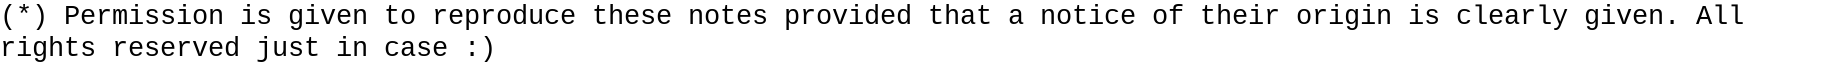
\includegraphics[width=0.8\linewidth]{img/image_2022-12-10-15-41-25.png}
			\caption{Excerpt from online course notes}
		\end{figure}
	\item Course will cover the following:
	 \begin{itemize}
	 	\item C to assembly
		\item How to build a processor that works
		\item Intro to processor optimizations
		\item Peripherals
		\item OS support (Maybe)
		\item (Maybe) Arithmetic circuits
		\item Use NIOS II and cover a little bit of RISC-V
	 \end{itemize}	
\end{itemize}



\subsubsection{Mark breakdown}

\begin{itemize}
	\item Labs 15\%
	\item project 5\%
	\item midterm  30\%
	\item Final 50\%
	\item All exams will be open notes/book/whatever except another person/service helping you.
\end{itemize}

\section{Preliminary}
\subsection{Lecture 2: Using binary quantities to represent other things}

Computers can represent information in bits; 0/1. 
Though they don't necessarily know or care what bits are, we may assign our own arbitrary meaning to them -- usually numbers with the help of positioning; the LSB represents $ 2^0 $ and so forth.

C types \marginnote{Or, just \texttt{\  ;;include <stdint.h>}...}
	\begin{itemize}
		\item int: 32b (word)
		\item char: 8b (byte)
		\item short: 16b (half word)
		\item long: 32b (word)
		\item long long: 64b
	\end{itemize}

Signed numbers may be represented in a number of ways.
\begin{itemize}
	\item Sign bit (make MSB represent positive or negative numbers and then the remaining $ n-1 $ bits represent the number. Con: hardware impl sucks because requires if/else
	\item Two's complement \sidenote{Flip bits, add one. Intuition; in 3 bit system, adding 7 to 1 would result in 8 which would get truncated to 0.}. Pro: only need to implement adders on hardware and then negative numbers will work just like any other except must be interpreted differently. Positive numbers would always start with a $ 0 $ and negatives would start with $ 1 $. So the range of possible values becomes $ -(2^{n-1}-1), +2^{n-1}-1$ 
\end{itemize}

Adding together binary numbers can also cause overflow; $ (A+B) \ge A, (A+B) \ge  B $ may not always be true.
Also, when we work with these types we always use all the bits. This has implications when working with values of different lengths.

\begin{itemize}
	\item \texttt{char b = -1}  \texttt{(1111 1111))}
	\item \texttt{short int c = -1}  \texttt{(0000 0000 0000 0001))}
	\item \texttt{a = b + c} \texttt{0000 0001 0000 0000 } 
	\item In order to deal with this we must \texttt{cast} the \texttt{char} to a \texttt{short int}. This is done via sign extension which prepends $ 0 $s or $ 1 $s \sidenote{two's complement} to the \texttt{char} so that math can be done on it.
\end{itemize}


\subsubsection{Floating Point Numbers}


Whereas fixed point numbers i.e. $ \$5.25 $ can be represented just as how an integer would be represented but with the understanding that the user would interpret it as having a decimal point somewhere that indicates the position of $ 2^0 $.
This decimal point would be the same for all numbers of that type, i.e. we could have a six bit number that has places $ 2^2 2^1 2^0 2^{-1} 2^{-2} $ 
This is common in embedded systems and how it is formatted isn't super clearly standardized.

\begin{lemma}
	Reference: \href{https://www.eecg.utoronto.ca/~moshovos/ECE352-2022/00.practice/What\%20Every\%20Computer\%20Scientist\%20Should\%20Know\%20About\%20Floating-Point\%20Arithmetic.htm}{What Every Computer Scientist Should Know About Floats}
\end{lemma}





\begin{definition}
	\textbf{IEEE 754 Floating Point}

	This is a single precision 32 bit float

	\begin{equation}
		\texttt{S  EEEEEEEE  MMMM MMMM MMMM MMMM MMMM MMM}
	\end{equation}
	

	The most significant \texttt{S} bit is the sign bit, bits 30 through 23 \texttt{E} form the exponent which is an unsigned integer, and 22 through 0 form the (\texttt{M})antissa. The number being represented can be found using the following:

	\begin{equation}
	(-1)^S \times 2 ^ {(E-127)} \times 1.\text{Mantissa}
		\label{eq:352:float32_eq}
	\end{equation}

	\begin{example}
		For example, given the following float:
		\begin{equation*}
			1\quad10000001\quad10000000000000000000000
		\end{equation*}
		
		So S = 1, E = 10000001 = 129 and Mantissa = 10000000000000000000000.
		The number is therefore

		\begin{equation}
			(-1^1) \times 2^{(129-127)} \times 1.10000000000000000000000 = -6.0
		\end{equation}
	\end{example}


	IEEE754 also defines 64 bit floating-point numbers. They behave the same except for now having an 11 bit exponent, the bias being 2047\mn{instead of 126}, and the mantissa having 52 bits\marginnote{In \texttt{c}, \texttt{float} is a 32 bit float and \texttt{double} is 64}.


	A few special cases are also available to represent other quantities

	\begin{itemize}
	\item If E=0, M non-zero, value=$(-1)^S \times 2^{-126} \times 0.M$ (denormals)
		\item If E=0, M zero and S=1, value=-0
		\item If E=0, M zero and S=0, value=0
		\item If E=1...1, M non-zero, value=NaN 'not a number`
		\item If E=1...1, M zero and S=1, value=-infinity
		\item If E=1...1, M zero and S=0, value=infinity
	\end{itemize}

	Floating-point numbers are inherently imprecise. Addition and subtract are inherently lossy; the mantissa window may not be large enough to capture the decimal points. Multiplication and division just creates a ton of numbers.
	\marginnote{There are more floating point formats introduced by nvidia and google such as a half-precision or 8-bit float designed to reduce memory use for machine learning}

	Converting real numbers to IEEE754 floats, here using 37.64 as an example, can be done as follows
	\begin{itemize}
		\item Repeatedly divide the part of the number $ >0 $ by $ 2 $ and get the remainders, i.e. 37/2 = 18, rem = 1 -> 18/2 = 0, rem = 0 -> 4/ 2 = 2, rem = 0, 2/2 = 1, rem = 0, 1/2 = 0, rem = 1. As a 2 bit number E is 100101. But we need to convert it to IEEE754 format with the exponent; E - 127 = 5, E = 132 = 1000 0100.
		\item Do the same for the part of the number past the decimal, but multiplying by two and checking if > 1: 0.64 * 2 = 1.28 -> 1, 0.28 * 2 = 0.56 -> 0, 0.56 * 2 = 1.12 -> 1 ... and so forth. At some point we will hit a cycle but we'll just take the $ N_{\text{mantissa}} $ of digits.
	\end{itemize}

	So the full number is $  0 1000 0100 0010 1101 0001 1110 1011 111 $
\end{definition}


\section{Memory and NIOS II}


\subsection{Lecture 3: Behavioural Model of Memory}


Computers can be described as a set of units, each of which interact with each other and the outside world in a specified way.
For example, modern computers tend to have memory units, processing units, display units, and so forth.
Each unit has a set of inputs and outputs, and a set of rules that govern how the unit behaves.
This gives the manufacturer flexibility in how they want to implement a unit, as long as the unit behaves as specified.
When designing these operational units it is important to strike a balance between functionality and specificity; if the unit is too specific it will be difficult to implement, but if it is too general it will be difficult to use.

\marginnote{\textbf{Specification} is the description of what an unit should do, and \textbf{implementation} is how it actually does it. For example, an \texttt{OR} gate can be specified as a truth table and then implemented via transistors or a person in a box.}

\subsubsection{Memory}
Memory is a unit that stores information and is usually represented as a vector of elements, usually a byte (8 bites).
Each element, or memory location, contains a binary quantity and has an associated \textit{address}.
The address is a number that uniquely identifies the location of the element in the vector, and is \textbf{permanently fixed} at time of manufacture.
Most systems are byte-addressable, meaning that there is an unique address for each byte in the memory.
The collection of all addresses is called the \textbf{address space} of the memory, which is typically a power of two.
Modern systems tend to be 32 or 64 bit, meaning that the address space is $ 2^{32} $ or $ 2^{64} $ elements long.

For each memory location there there are two operations available
\begin{itemize}
	\item \textbf{Read}: Read the value stored at a given address
	\item \textbf{Write}: Write a value to a given address
\end{itemize}


Typical memory behaviour models define that the order of memory operations matters, i.e. 

\begin{enumerate}
	\item \texttt{store 0x10, 0xf0} 
	\item \texttt{store 0x20, 0xf0} 
\end{enumerate}

We would see that \texttt{0xf0} contains the value \texttt{0x20} and not \texttt{0x10} due to the sequential execution model.
Memory that adheres to the sequential model offers operations that are \textbf{atomic}; the operations are performed on its own with no interaction or overlap with anything else.



\begin{figure}[H]
	\centering
	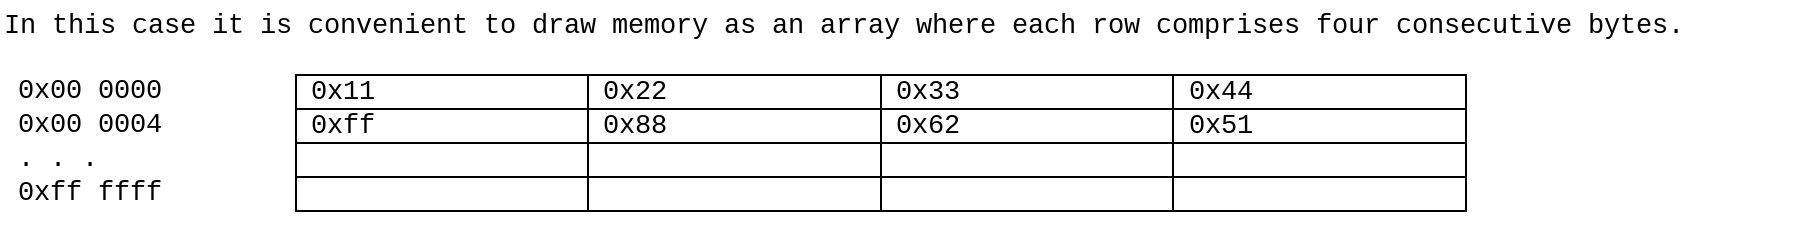
\includegraphics[width=\linewidth]{img/image_2022-09-16-02-10-27.png}
\end{figure}

Systems are generally also addressable by words, halfwords, and bytes.
Different architectures have different constraints on allowing unaligned access\sidenote{Aligned access only means to allow [only] reads or writes for a data size i.e. halfword to an address divisible by the size of said data type. For example an longword access on our development board would be at an address divisible by $ 4 $}

\textbf{Endianness} refers to the order in which bytes are stored in memory. Though some processors are big-endian, most modern processors are little-endian. The NIOS II used for this course is little-endian. 

\begin{figure}[H]
	\centering
	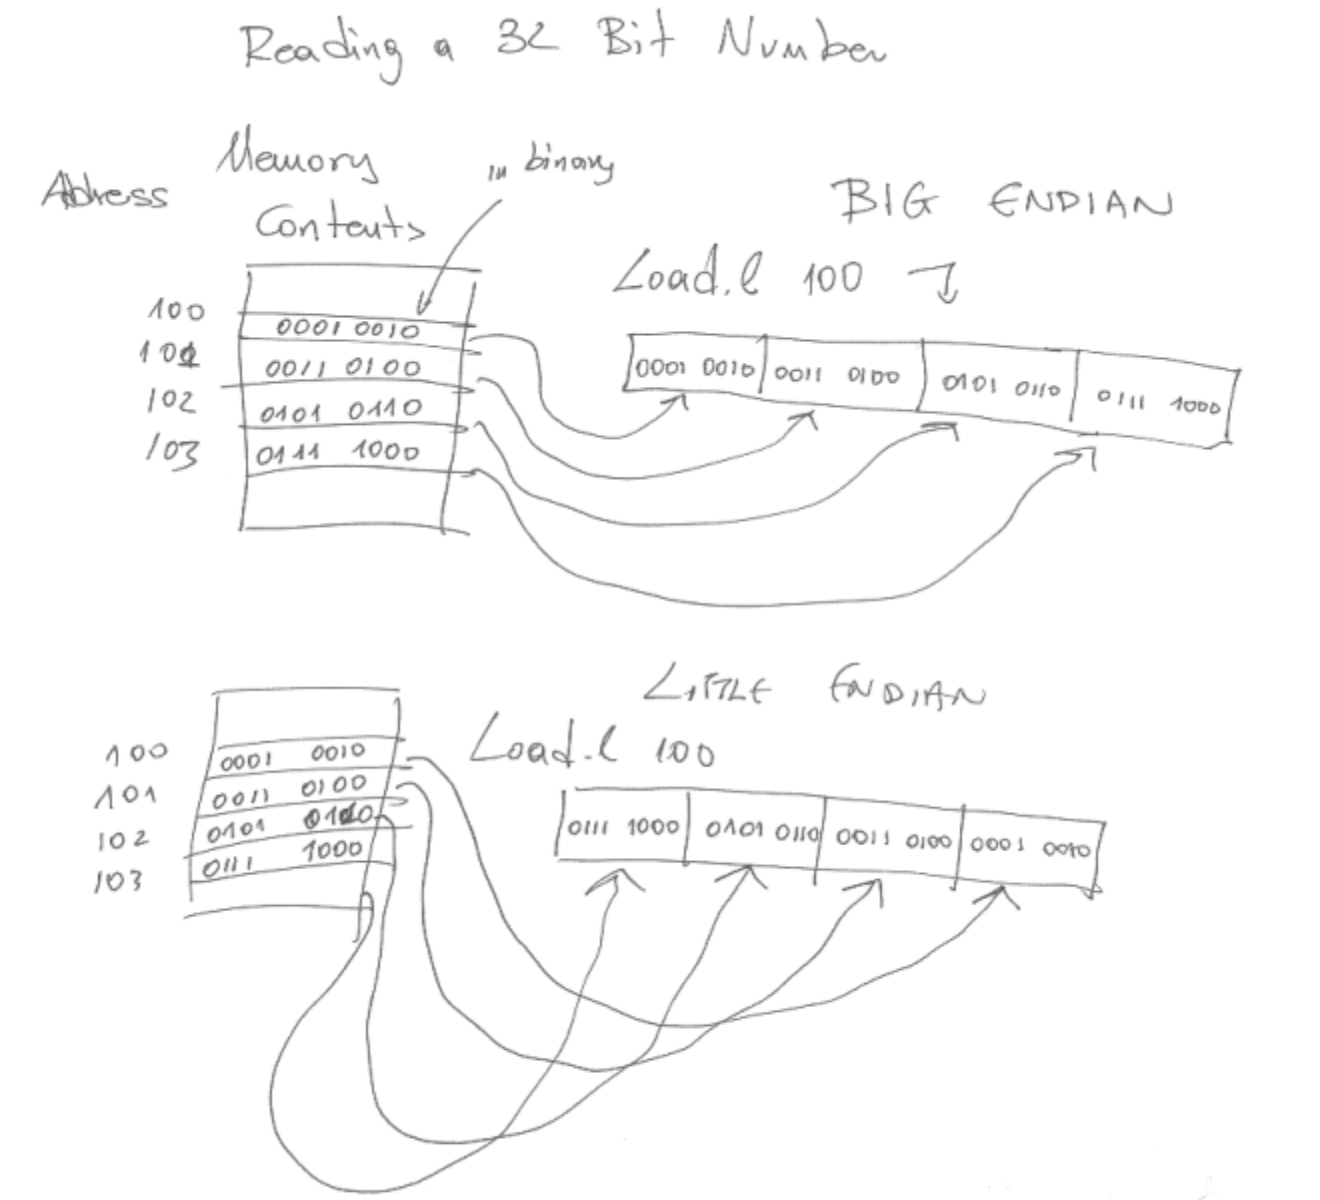
\includegraphics[width=0.8\linewidth]{img/image_2022-09-16-02-16-30.png}
\end{figure}

\subsubsection{Physical Interface}

What physical interfaces would be necessary to implement this behavioural model? 

Given a summary of requirements as follows:

\begin{enumerate}
	\item Read and write operations
	\item Addressable by byte, word, longword
	\item 24 bit address
	\item 32 bit for writing
	\item 32 bit for reading
	\item signal for do nothing
\end{enumerate}


A single bit signal can be used to indicate whether the memory is reading or writing, and a two bit signal can be used to specify if we're interested in addressing by byte, word, or longword.
The address is 24 bits, so we need 24 address lines.
As for reading/writing data, we have the option of having two 32 bit data lines, or multiplexing a single 32 bit line.
A single bit signal can be used to indicate to do nothing or not. \marginnote{The use of a single bit signal to indicate `do nothing' is necessary because a physical device won't be able to change all signals instantaneously, so we use it to tell the memory to wait until these transient effects die off}

One way of multiplexing the data lines is to use a tri-state buffer, which is a buffer that can be enabled or disabled.
When enabled, the buffer acts as a normal buffer, but when disabled, the output is disconnected from the input.
On the other hand this means that our memory chip would not support simultaneous reads or writes.




\begin{figure}[H]
	\centering
	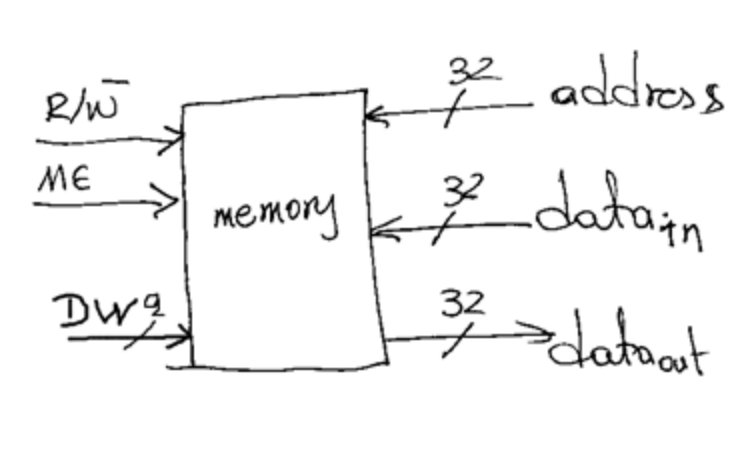
\includegraphics[width=0.8\linewidth]{img/image_2022-09-16-02-18-16.png}
\end{figure}

\subsection{Lecture 4: NIOS II Programming Model}

The NIOS II assumes a \texttt{32-bit} address space where each address holds a single byte.
Each byte is addressable, and three data types are supported. Halfword and word accesses must be aligned.

\begin{itemize}
	\item \textbf{Byte}: 8 bits
	\item \textbf{Halfword}: 16 bits
	\item \textbf{Word}: 32 bits
\end{itemize}

The NIOS II also has a set of registers

\begin{itemize}
	\item 32 general purpose 32 bit registers
		\begin{itemize}
			\item \texttt{r0} is always zero\marginnote{Many operations can be synthesized using another operation involving zero, i.e. assignment \texttt{A=B} can be implemented as \texttt{A = B + 0} }
		\end{itemize}
	\item 6 control registers, 32 bits each
	\item Program counter (PC), 32 bits
\end{itemize}

There are certain conventions for the use of registers, which are as follows:
\begin{figure}[H]
	\centering
	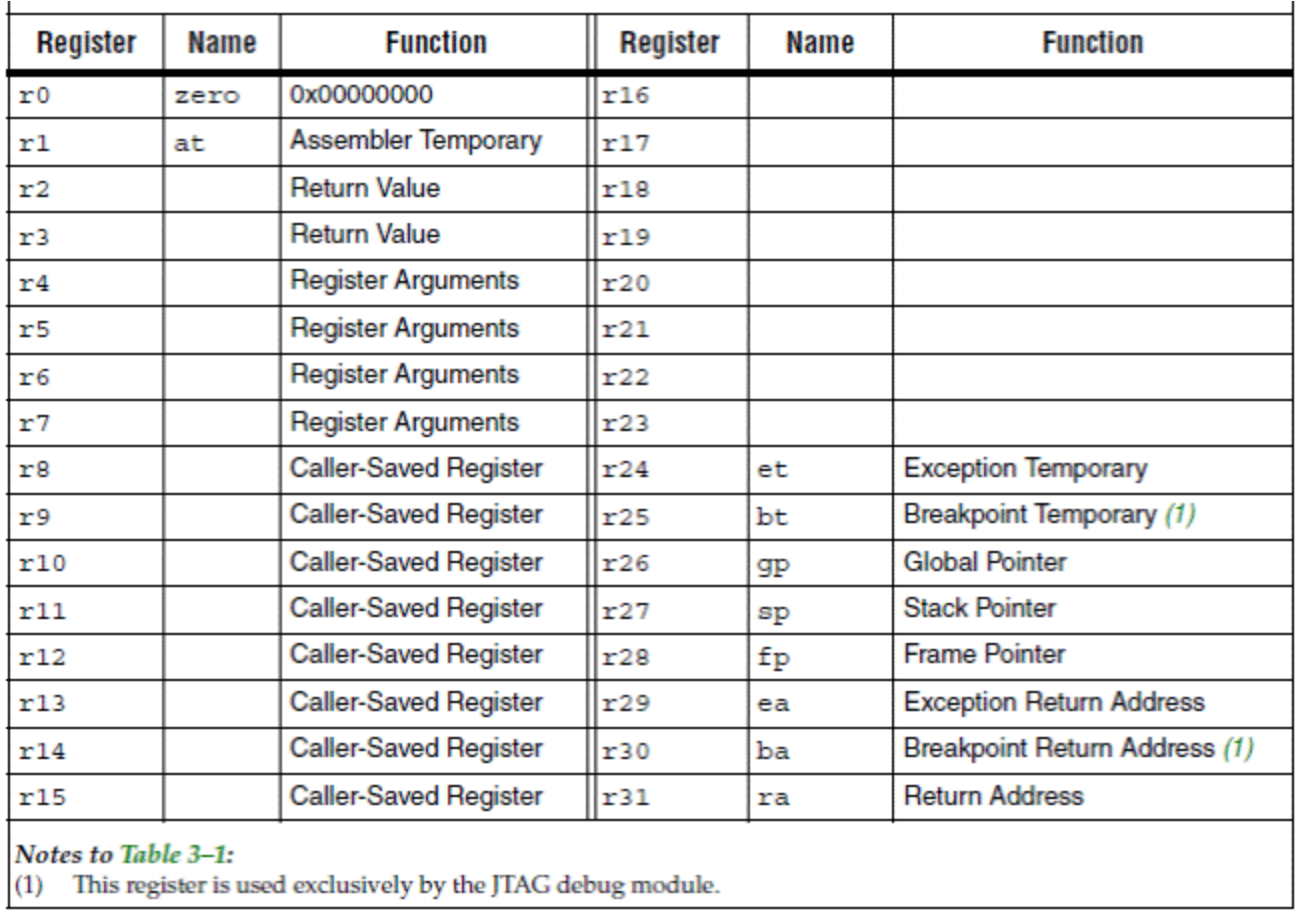
\includegraphics[width=0.8\linewidth]{img/image_2022-09-16-17-17-34.png}
\end{figure}

\subsubsection{Adding Two Numbers}
As an exercise, let's see how we can implement the following piece of code in NIOS II assembly

\begin{listing}[H]
\begin{minted}{c}
unsigned int a = 0x00000000;
unsigned int b = 0x00000001;
unsigned int c = 0x00000002;

a = b + c;
\end{minted}
\end{listing}


\textbf{Register-only version} 

\marginnote{\texttt{addi} stands for `add intermediate', the only difference being that the second operand is a number. It is used to set a constant}

\begin{listing}[H]
\begin{minted}{gas}
addi r9, r0, 0x1
addi r10, r0, 0x2
add r9, r10, r11
\end{minted}
\end{listing}

In general, most instructions take the form of \texttt{operation destination, source1, source2}.


Breaking it down even further we can see that these assembly instructions actually perform a number of steps

\begin{listing}[H]
\begin{minted}{gas}
addi r9, r0, 0x1
	; 1. read r0
	; 2. Add value read in step 1 with 0x1
	; 3. Write result of step 2 to r9
	; 4. increment PC to next instruction
addi r10, r0, 0x2
	; 1. read r0
	; 2. Add value read in step 1 with 0x2
	; 3. Write result of step 2 to r10
	; 4. increment PC to next instruction
add r9, r10, r11
	; 1. read r10
	; 2. read r11
	; 3. Add values read in steps 1 and 2
	; 4. Write result of step 3 to r8
	; 5. increment PC to next instruction
\end{minted}
\end{listing}


What about 32 bit constants? An unfortunate quirk is that \texttt{addi} only supports 16 bit constants, so we need to use \texttt{ori} to set the upper 16 bits of the register.


\begin{listing}[H]
\begin{minted}{gas}
movhi r9, 0x1122
	; Sets the upper 16 bits of r9 to 0x1122
	; and the lower 16 bits to zero
ori r9, r9, 0x3344
	; bitwise OR the value in r9 with 0x3344
	; which will set the lower 16 bits to 0x3344
\end{minted}
\end{listing}

This is a PITA so NIOS II offers a few pseudo-instructions to make this easier




\begin{listing}[H]
\begin{minted}{gas}
movi rX, Imm16
	; sets rX to the sign-extended (signed) 16 bit immediate
movui rX, Imm16
	; sets rX to a zero-extended unsigned 16 bit immediate
movia rX, Imm32
	; sets rX to a 32 bit immediate
\end{minted}
\end{listing}

{\let\thefootnote\relax\footnote{
	\begin{itemize}
		\item Footnote1: \texttt{movia} does not use the \texttt{movhi} and \texttt{ori} instructions to create a 32-bit immediate but rather a \texttt{movhi} and a \texttt{addia}.
\texttt{addi}  will sign extend it's 16-bit field so some adjustment might be needed for whatever is being passed to \texttt{movhi}.
		\item Footnote2: movhi r9, \%hi(0x11223344) is equivalent to movhi r9, 0x1122. Ori r9, \%lo(0x11223344) is equivalent to ori 9, 0x3344. That is, \%hi(Imm32) returns the upper 16-bits of Imm32 and \%lo(Imm32) the lower 16 bits.
		\item Footnote3: movhi r9, \%hiadj(0x11223344) followed by addi r1, \%lo(0x11223344) is the correct way of creating a 32-bit immediate using movhi and addi. \%hiadj(Imm32) returns the upper 16 bits of the immediate  as-is or incremented by 1 if bit 15 is 1. Think why this is necessary based on footnote 1.
		\item Footnote4: \%hi(), \%lo(), and \%hiadj() are macros supported by the assembler. They are not NIOS II instructions. They get parsed during compile time. 
	\end{itemize}
}}


\subsubsection{Adding two numbers using memory}

NIOS II is a load/store architecture which means that all data manipulation happens only in registers.


\begin{listing}[H]
\begin{minted}{gas}
; read b from memory into r9
movhi r11, 0x0020
ori   r11, r11, 0x0004
ldw   r9, 0x0(r11)

; read c from memory into r10
movhi r11, 0x0020
ori   r11, 0x0008
ldw   r10, 0x0(r11)

; add, then store into r8
add   r8, r9, r10

; store r8 into memory
movhi r11, 0x0020
ori   r11, r11, 0x0000
stw   r8, 0x0(r11)
\end{minted}
\end{listing}


The new instructions introduced here are


\begin{listing}[H]
\begin{minted}{gas}
ldw rX, Imm16(rY) ;; 'load word' from memory
;; rX, rY registers, Imm16 is a 16 bit immediate
;; TLDR; Rx = mem[rY + sign-extended(Imm16)]
; 1. read rY
; 2. sign-extend Imm16 to 32bits
; 3. adds the result of step 1 and 2
; 4. reads from memory a word (32 bit) using the result of step 3 as the address
; 5. write the result of step 4 to rX
\end{minted}
\end{listing}

\begin{listing}[H]
\begin{minted}{gas}
stw rX, Imm16(rY) ;; 'store word' to memory
;; rX, rY registers, Imm16 is a 16 bit immediate
;; TLDR; mem[rY + sign-extended(Imm16)] = rX
; 1. read rY
; 2. sign-extend Imm16 to 32bits
; 3. adds the result of step 1 and 2
; 4. write to memory rX using the result of step 3 as the address
\end{minted}
\end{listing}

This can be simplified using the \texttt{movia} macro

\begin{listing}[H]
\begin{minted}{gas}
movia r11, 0x200004
ldw   r9, 0x0(r11)
movia r11, 0x200008
ldw   r10, 0x0(r11)
add   r8, r9, r10
movia r11, 0x200000
stw   r8, 0x0(r11)
\end{minted}
\end{listing}


In this lecture so far we have seen three addressing modes

\begin{enumerate}
	\item Register addressing, i.e. \texttt{rX} 
	\item Immediate addressing, i.e. \texttt{Imm16}
	\item Register indirect addressing with displacement, i.e. \texttt{Imm16(rY)}. This is how we calculate the referenced memory address. Register indirect refers to using a register's value to refer to memory, and `displacement' refers to adding a constant prior to using the register value to access memory. Register indirect addressing is where we use a displacement of 0.
\end{enumerate}


We can exploit register indirect addressing with displacement.

\begin{listing}[H]
\begin{minted}{gas}
movhi r11, 0x0020
ori   r11, r11, 0x0004
ldw   r9, 0x0(r11)
;; can be replaced with
movhi r11, 0x0020
ldw r9, 0x4(r11)
\end{minted}
\end{listing}

Note that the value of \texttt{r11} does not change since the subsequent operations use an offset to that value.

Generally when we want to read memory from \texttt{A} we can use

\begin{listing}[H]
\begin{minted}{gas}
movhi r11, (upper 16 bits of A)
ori   r9, r11, (lower 16 bits of A)
\end{minted}
\end{listing}


Care must be taken when the 16th bit of \texttt{A}  is 1 since the addition that \texttt{ldw} performs will sign extend it to be a negative number, i.e. 

\begin{listing}[H]
	\begin{minted}{gas}
movhi r11, 0x0020
ldw r9, 0x8000(r11)
;; this is incorrect because
;; will extend to 0xFFFF8000, which would result
;; in a final address of 0x001F800
\end{minted}
\end{listing}


This is where the macros \texttt{\%hiadj(Imm32)}  and \texttt{\%lo(Imm32)} come in handy, since they will add 1 to the values if bit 15 of Imm32 is 1. 
This results in code that looks like this:


\begin{listing}[H]
	\begin{minted}{gas}
movhi r11, %hiadj(0x208000)
ldw r9, %lo(0x2080000)(r11)
;; will extend to 0xFFFF8000, which would result
;; in a final address of 0x001F800
\end{minted}
\end{listing}


\section{Assembly Basics}
\subsection{Lecture 5: Simple Control Flow}

We have prior worked with straight-line sequences.
In this lecture we will look at how to add control flow to our programs, i.e if-then-else, etc.


\marginnote{The \texttt{data} section contains stuff that you want to be initialized for you before the entry point of the program is called, e.g. global variables. This segment as a fixed size. The \texttt{text} or \texttt{code} segment contains executable instructions (typically read-only, unless the architecture allows self-modifying code) and typically resides in the lower parts of memory. \texttt{bss} contains static and global variables which are zero-initialized; usually used for uninitialized data}

A pseudo-c program will be rewritten in assembly to illustrate the concepts.

\begin{listing}[H]
\begin{minted}{c}
unsigned int a = 0x00000000;
unsigned int b = 0x11223344;
unsigned int c = 0x22334455;

if (b == 0)
then a = b + c;
else a = b – c;

\end{minted}
\end{listing}

\begin{listing}[H]
\begin{minted}{gas}
      .section .data
va:   .long 0x0
vb:   .long 0x11223344
vc:   .long 0x55667788
 

main:
      movia r11, va
      ldw   r9, 4(r11)
      beq   r9, r0, then
else:
      ldw   r10, 8(r11)
      sub   r8, r9, r10
      stw   r8, 0(r11)
      beq   r0, r0, after

then:
      ldw   r10, 8(r11)
      add   r8, r9, r10
      stwio r8, 0(r11)
after:
\end{minted}
\end{listing}
\begin{definition}

	We encounter two new instructions in this snippet.
\begin{itemize}
	\item \texttt{sub} is a subtraction instruction
	\item \texttt{beq}: a branch-if-equals instruction
\end{itemize}

The \texttt{beq} instruction takes the general form 

\texttt{beq RX, rY, label}. 

This instruction will compare the values of $ rX $ and $ rY $ and if the condition is true then the program counter will jump to the destination label. 
When the branch changes the program counter it is called a taken branch, otherwise it is non-taken. Non-taken branches fall through to the next instructions. 

\begin{blockquote}
	Note: whereas the assembly \texttt{beq} command is written as a comparison with a label to jump to, in the NIOSII instruction the destination is encoded relative to the instruction location with a 16-bit displacement constant. The displacement is therefore calculated as $ PC + 4 + \text{displacement} $, meaning that we can jump at most $ +32774, -32772 $ bytes\mn{16 bit signed constant+4, with 4-byte alignment since instructions are 4 bytes long.} from the current program counter. The compiler will complain if the branch cannot be implemented.


	Encoding is as follows: 

	\texttt{AAAAA BBBBB IIIIIIIIIIIIIIII 0x26}.

	where $ A $, $ B $ are register names (hence 5 bit), $ I $ is a 16 bit immediate value, and $ 0x26 $ is the branch type, in this case $ beq $  


	Most branches tend to be branch backwards because of loops.
\end{blockquote}


Other branch instructions include


% TODO (ihasdapie): Finish up this list & cleanup
\begin{itemize}
	\item \texttt{br}: always/unconditional branch
	\item \texttt{bne}: branch if not equal
	\item \texttt{blt}: branch if less than, w/ signed comparison
	\item \texttt{bltu}: branch if less than, w/ unsigned comparison
	\item \texttt{bgt}: branch if greater than, w/ signed comparison
	\item \texttt{bgtu}: branch if greater than, w/ unsigned comparison


\end{itemize}


\end{definition}






\begin{listing}[H]
\begin{minted}{gas}
	.data
	.align 4 ;; Align to word size addresses which are faster to access
a: .word 0
b: .word 0x11223344
c: .word 0x55667788
	.text
	movia r11, a  ;; moves the address of a into r11
	ldw r9, 4(r11) ;; loads the value at address a+4 into r9
	ldw r10, 8(r11)
	add r8, r9, r10
	stw r8, 0(r11)
\end{minted}
\end{listing}






\subsection{Lecture 6, 7: For loops and arrays}

How can we implement the following in assembly?

\begin{listing}[H]
\begin{minted}{c}
short arr[5] = { 1, 2, 3, 4, 5 }; // an array of word values (16 bit)
short n = 5;            // the number of elements in the array
short sum = 0;
 
for (i = 0; i  < n; i++)
   sum = sum + arr[i];
\end{minted}
\end{listing}


Arrays are typically implemented at the machine level as a contiguous block of memory.
\marginnote{Generally element \texttt{a[i]} is at address \texttt{\&a[0] + sizeof(TYPE) * i}    }

\begin{listing}[H]
	\begin{minted}{gas}
		.data
		.align 1
arr .hword 1,2,3,4,5
n   .hword 5
sum .hword 0
	\end{minted}
	\caption{Creating a static array in assembly}
\end{listing}

Multidimensional arrays are handled by having an array of pointers to arrays and dereferencing twice to arrive at the desired memory location.
Alternatively we can allocate a $ 1x(m \cdot  n) $ chunk of memory and then address it as $ a[i][j] = a[i \cdot n + j] $.
\marginnote{\texttt{c} and pascal and other modern programming languages store arrays in row-major order, i.e. consecutive elements in a row are place together in memory. FORTRAN uses column-major.}





As for the for loop, let's look at at what \texttt{c} does first.

\begin{listing}[H]
\begin{minted}{c}
for (init; cond; post)
	body
\end{minted}
\caption{General form of a \texttt{c} for loop}
\end{listing}


Breaking it down a little more into atomic steps


\begin{listing}[H]
\begin{minted}{c}
INIT
if (!COND), we are done
BODY
POST
GOTO line 2
\end{minted}
\caption{General form of a \texttt{c} for loop}
\end{listing}

Let's now rewrite this in assembly

\begin{listing}[H]
\begin{minted}{gas}
		.text
forloop:
	add r8, r0, r0 ;; INIT
	movia r9, n ;; set COND, i.e. the n that we compare i to. See: loop invarient :)
	ldh r9, 0(r9)
;; movhi r9, %hiadj(n)
;; ldh r9, %lo(n)(r9) ;; this code block is a shorter piece with the same effect
loop:
	bge r8, r9, endloop ;; test condition for when we are done
	;; body goes here
	;; let's use r10 to store the running sum at in the end we can load it to memory
	movia r11, arr ;; load the address of arr[0] into r11
	;; add the index to the address of arr[0]; &arr + i
	add r11, r11, r8
	;; add again; &arr + i + i = &arr + 2i
	add r11, r11, r8
	ldhio r12, 0(r11) ;; r12 = arr[i]
	add r10, r10, r12 ;; r[10] += arr[i]
	
	addi r8, r8, 1 ;; POST i.e. r8 += 1
	br loop
endloop:
	movia r11, sum
	sth r12, 0(r11) ;; write the sum to memory
\end{minted}
\end{listing}


A similar approach can be taken for while loops.


\begin{listing}[H]
\begin{minted}{gas}
.text
    
add       r8, r0, r0 ;; zero out r8
movia     r9, n ;; assumes n >= 1
ldh       r9, 0(r9) ;; loads condition
    
doloop:  
					movia r11, arr ;; grab address of arr[0]
					add  r11, r11, r8 
					add  r11, r11, r8 ;; grab addr of arr[i]
					ldh  r12, 0(r11) ;; load arr[i] into r12
					add   r10, r10, r12 ;; add arr[i] to sum
 
          addi r8, r8, 1 ;; increment i
          blt  r8, r9, doloop ;; evaluate loop condition
endloop:
          movia r11, sum
          sth  r12, 0(r11)  ;; write the sum into memory
\end{minted}
\end{listing}


\begin{blockquote}
	\texttt{gcc} is not a compiler by itself: it actually orchestrates and calls out a lot of other things

	\begin{enumerate}
	\item \texttt{cpp}: the C preprocessor, $    f.c \to  f.i $  ; dealing with \texttt{\  ;; defines}, etc. Inspect via \texttt{gcc -E} 
	\item \texttt{gcc -s f.i}: the \texttt{cc}, the c compiler $ f.i \to f.s $  : parse pure c from preprocessor and spew out assembly code
	\item \texttt{as}: the assembler, $ f.s \to f.o $:   to turn assembly to machine code, creating objects ready for linkage
	\item \texttt{ld}: the linker, $ f.o \to f $:  link together all the objects into a single executable. Looks through \texttt{LDPATH} to look for symbols to link. \mn{There is static and dynamic linking; static meaning that everything is inside. These days most are dynamically linked which can grab symbols from shared libraries (\texttt{.so}) right before/during runtime}
	\end{enumerate}
\end{blockquote}



\subsection{Lecture 8: Subroutines}

A subroutine (or how we more commonly understand them, function calls), is a way to break up a program into smaller pieces and is a core part of structured programming.

Let's look at how we can implement the following in assembly

\begin{listing}[H]
\begin{minted}{c}
int add3(int a, int b, int c){
	return a+b+c;
}
\end{minted}
\end{listing}

First, for \texttt{c}  subroutines to work as intended they must:

\begin{enumerate}
	\item Be callable from anywherei n the program
	\item Be able to pass unique parameters across different subroutine invocations
	\item Be able to return a value to the caller
	\item Must be able to change control flow such that it goes back to the point where it was called
\end{enumerate}

This leads to a number of questions:

\begin{enumerate}
	\item How does the subroutine return to the caller?
	\item how does it return a value?
	\item How do we pass arguments?
	\item What about local memory?
	\item What happens to registers when we call a subroutine?
\end{enumerate}


These issues are addressed through a set of implementation-specific (though largely universal) rules that all valid subroutines must follow. These are called \textbf{calling conventions}.



\begin{definition}
	A key concept in subroutine calling is the \textbf{stack frame}. As for how stacks work/are implemented that is a google search away.

	A stack has the following operations defined:

		\begin{enumerate}
			\item push: put a value on the top of the stack
			\item pop: remove the top value from the stack
			\item peek (distance): look at the value at a certain distance from the top of the stack
		\end{enumerate}

\end{definition}


	The NIOS II stores it's stack pointer, or the address to the top of the stack, in \texttt{r27}, i.e. the stack pointer \texttt{sp}.
	The \texttt{sp}  starts at the top of the stack (highest address value) and then the stack grows downwards to lower addresses.\sn{Conversely the heap (commonly used for dynamic memory allocation) grows upwards towards higher addresses. The stack and heap are commonly implemented such that they grow towards each other}
	There is no way to represent an empty stack in NIOS II; \texttt{r27} will always contain a valid pointer address.
	\sidenote{An element is in the stack if it's address is greater than \texttt{sp} }


\begin{definition}
	\textbf{push}  
	\begin{listing}[H]
	\begin{minted}{gas}
	;; push r9 -> stack
	subi sp, sp, 4 ;; grow stack by a long word
	;; (recall: grow downwards)
	stw r9, 0(sp) ;; save value of r9 to sp
	\end{minted}
	\end{listing}


	\textbf{pop}  
	\begin{listing}[H]
	\begin{minted}{gas}
	;; pop top of stack and return to r9
	ldw r9, 0(sp) ;; read top value
	addi sp, sp, 4 ;; increment sp; remove top elem
	\end{minted}
	\end{listing}

	\textbf{top}  
	\begin{listing}[H]
	\begin{minted}{gas}
	// access ith elem, assuming index in r9
	add r9, r9, r9 ;; assume r9 contains nedex
	add r9, r9, r9 // r9 = 4 * i
	add r9, sp, r9 ;; sp + 4*i
	ldw r9, 0(r9) // return value of ith element into r9
	\end{minted}
	\end{listing}
\end{definition}


\textbf{Calling a subroutine and having it return to the caller}  


\marginnote{\texttt{r31} is commonly used as the return address pointer and is aliased as \texttt{ra} }
The stack is used to implement this behaviour.
If a function will be calling another it has to save the \texttt{ra}  value on the stack in the beginning and restore it from the stack prior to returning.

Consider the following pseudo \texttt{c} code

\begin{listing}[H]
\begin{minted}{c}
boo_calls(){
	coo();
	doo();
	return;
}

coo(){
	doo();
	return;
}
doo(){
	return;
}
\end{minted}
\end{listing}

The NIOS II code would be as follows

\marginnote{Note that \texttt{ret} transfers execution to the address in \texttt{ra}  }
\begin{listing}[H]
\begin{minted}{gas}

	.text
boo:  ;; boo will be making calls, so it first pushes the ra value on the stack   
	subi sp, sp, 4  
	stw ra,0(sp)  ;; push the return address onto the stack


	call coo  ;; resume execution at coo, ra = PC + 4 = boo_ret1
boo_ret1:
	call doo  ;; continue execution at doo, ra = PC + 4 = boo_ret2

boo_ret2:                                        
	ldw  ra, 0(sp)  ;; pop return address from the stack
	addi sp, sp, 4
	ret  ;; resume execution at ra, which would be the return address from the 
	;; stack we just popped
coo:
	subi  sp, sp, 4 
	stw   ra,0(sp)  ;; push the return address onto the stack
	call  doo  ;; resume execution at coo, ra = PC + 4 = coo_ret

coo_ret:
	ldw  ra, 0(sp)  ;; pop return address of boo from the stack
	addi sp, sp, 4
	ret  ;; resume execution there

doo:  ;; doo will not be making any calls, no need to save ra on the stack
	ret  ;; just return to whoever called 
\end{minted}
\end{listing}





\begin{figure}[H]
	\centering
	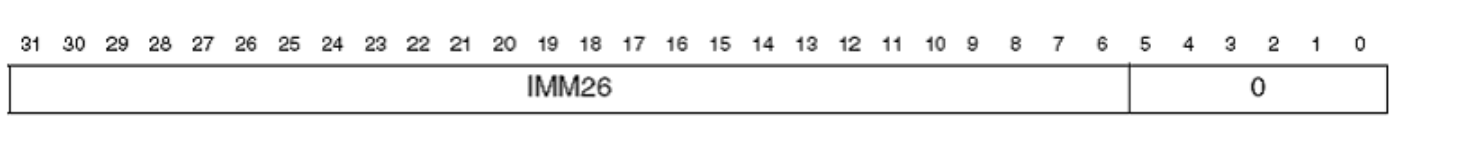
\includegraphics[width=0.8\linewidth]{img/image_2022-09-26-14-48-27.png}
	\caption{The call instruction accepts a label as the 2nd argument which is encoded as a 26 bit immediate. This limits the called function to be within 256 MB of the caller; the actual target is the immediate multiplied by 4 and then concatenating with the program counter, i.e. $ PC_{31\ldots28} = IMM26 * 4 $ }
\end{figure}

Note: we can look at executables with \texttt{objdump -d}. 

Example:


\begin{listing}[H]
\begin{minted}{c}

#include <stdio.h>
int main () {
	printf("hello world");
}

\end{minted}
\end{listing}

\begin{listing}[H]
\begin{minted}{gas}

hello_world:     file format elf64-x86-64


Disassembly of section .init:

0000000000001000 <_init>:
    1000:	f3 0f 1e fa          	endbr64
    1004:	48 83 ec 08          	sub    $0x8,%rsp
    1008:	48 8b 05 c1 2f 00 00 	mov    0x2fc1(%rip),%rax        # 3fd0 <__gmon_start__@Base>
    100f:	48 85 c0             	test   %rax,%rax
    1012:	74 02                	je     1016 <_init+0x16>
    1014:	ff d0                	call   *%rax
    1016:	48 83 c4 08          	add    $0x8,%rsp
    101a:	c3                   	ret

Disassembly of section .plt:

0000000000001020 <printf@plt-0x10>:
    1020:	ff 35 ca 2f 00 00    	push   0x2fca(%rip)        # 3ff0 <_GLOBAL_OFFSET_TABLE_+0x8>
    1026:	ff 25 cc 2f 00 00    	jmp    *0x2fcc(%rip)        # 3ff8 <_GLOBAL_OFFSET_TABLE_+0x10>
    102c:	0f 1f 40 00          	nopl   0x0(%rax)

0000000000001030 <printf@plt>:
    1030:	ff 25 ca 2f 00 00    	jmp    *0x2fca(%rip)        # 4000 <printf@GLIBC_2.2.5>
    1036:	68 00 00 00 00       	push   $0x0
    103b:	e9 e0 ff ff ff       	jmp    1020 <_init+0x20>

Disassembly of section .text:

0000000000001040 <_start>:
    1040:	f3 0f 1e fa          	endbr64
    1044:	31 ed                	xor    %ebp,%ebp
    1046:	49 89 d1             	mov    %rdx,%r9
    1049:	5e                   	pop    %rsi
    104a:	48 89 e2             	mov    %rsp,%rdx
    104d:	48 83 e4 f0          	and    $0xfffffffffffffff0,%rsp
    1051:	50                   	push   %rax
    1052:	54                   	push   %rsp
    1053:	45 31 c0             	xor    %r8d,%r8d
    1056:	31 c9                	xor    %ecx,%ecx
    1058:	48 8d 3d da 00 00 00 	lea    0xda(%rip),%rdi        # 1139 <main>
    105f:	ff 15 5b 2f 00 00    	call   *0x2f5b(%rip)        # 3fc0 <__libc_start_main@GLIBC_2.34>
    1065:	f4                   	hlt
    1066:	66 2e 0f 1f 84 00 00 	cs nopw 0x0(%rax,%rax,1)
    106d:	00 00 00 

		;; and this goes on for a while loading in the .so & printf
\end{minted}
\end{listing}


And more assembly later ... 



\begin{listing}[H]
\begin{minted}{gas}

0000000000001139 <main>:
    1139:	55                   	push   %rbp
    113a:	48 89 e5             	mov    %rsp,%rbp
    113d:	48 8d 05 c0 0e 00 00 	lea    0xec0(%rip),%rax        # 2004 <_IO_stdin_used+0x4>
    1144:	48 89 c7             	mov    %rax,%rdi
    1147:	b8 00 00 00 00       	mov    $0x0,%eax
    114c:	e8 df fe ff ff       	call   1030 <printf@plt>
    1151:	b8 00 00 00 00       	mov    $0x0,%eax
    1156:	5d                   	pop    %rbp
    1157:	c3                   	ret

Disassembly of section .fini:

0000000000001158 <_fini>:
    1158:	f3 0f 1e fa          	endbr64
    115c:	48 83 ec 08          	sub    $0x8,%rsp
    1160:	48 83 c4 08          	add    $0x8,%rsp
    1164:	c3                   	ret


\end{minted}
\end{listing}

























\subsection{Lecture 9}

We've seen how to call and return from subroutines -- but what about passing arguments and returning values?
\marginnote{The following calling convention is the one used by gcc for the NIOS II family}
For this lecture we'll assume that only words are returned from and passed to subroutines, but other data types and structs can be used as well.


\begin{itemize}
	\item Return value is passed in \texttt{r2}\mn{only one return value can be given; multiple can be encoded via structures or ptrs etc}
	\item First four parameters are passed in \texttt{r4, r5, r6, r7} 
	\item Additional parameters are pushed onto the stack \textit{in order} 
		\begin{itemize}
			\item We push the last argument to the stack first and so forth such that the first non-register argument (the 5th one) is the first to be popped off once we enter the function.
		\end{itemize}
\end{itemize}

Consider a function which takes seven integers and adds them together.

\begin{listing}[H]
\begin{minted}{gas}
	.data
sum: .word 0
	.text
main:

addi sp, sp, -4
stw ra, 0(sp);
;; return address ptr (ra) is pushed onto the stack

;; fill first 4 args
movi r4, 1
movi r5, 2
movi r6, 3
movi r7, 4

;; allocated for arguments 5-7
addi sp, sp, -12 ;; 3 words * 4 byte


;; push arguments 5-7 onto the stack
;; note order; <top> 5, 6, 7
movi r2, 7
stw r2, 8(sp)

movi r2, 6
stw r2, 4(sp)

movi r3, 5
stw r2, 0(sp)

call add7

add7:
	add r2, r4, r5    # add the first two arguments and place the sum into r2
	add r2, r2, r6    # add the third argument to r2
	add r2, r2, r7    # add the fourth argument to r2
	ldw r7, 0(sp)     # read the fifth argument from the stack
	add r2, r2, r7    # add to r2
	ldw r7, 4(sp)     # read the sixth argument from the stack
	add r2, r2, r7    # add to r2
	ldw r7, 8(sp)     # read the seventh argument from the stack
	add r2, r2, r7    # add to r2 (return value in r2 by convention)
	 ret
;; and then do the cleanup etc
\end{minted}
\end{listing}

Note that in reality \texttt{gcc}   will actually preallocate all the memory needed by the function before the function is called. So instead of allocating 12 bytes (3x 1 word arguments) as it does on line 17, it will actually allocate 16 bytes because we need to store the return address.

The allocated stack frame for the function will be the largest of any function being called from it.

For example,

\begin{listing}[H]
\begin{minted}{c}
int main(){
	foo(1,2,3);
	boo(1,2,3,4,5,6,7,8);
}
\end{minted}
\end{listing}

Boo has the maximum number of arguments, so we'll need to allocate $ 8-4=4 $ words on the stack for the arguments and the return address -- $5*4=20$ bytes. This results in

\begin{listing}[H]
\begin{minted}{gas}
;; prologue
addi sp, sp, -20
stw, ra, 16(s0)  ;; note little-endian and remaining 16 bytes for 4 argument words

;; epilogue
ldw ra, 16(sp) // pop return addr from stack
addi sp, sp, 20;
\end{minted}
\end{listing}












\subsection{Lecture 10: Recursive Subroutines}

Consider this code block that computes the Ackerman function


\begin{listing}[H]
\begin{minted}{c}
int Ackerman(unsigned int x, unsigned int y)
{
	if (x==0) return y+1;
	if (y==0) return Ackerman(x-1, 1);
	return Ackerman(x-1, Ackerman(x, y-1));
}
\end{minted}
\end{listing}

This function is interesting to implement because of it's recursive nature.


Breaking it down a little more,
\begin{listing}[H]
\begin{minted}{c}
int Ackerman(unsigned int x, unsigned int y)
{
	if (x==0) return y+1;
	if (y==0) return Ackerman(x-1, 1);
	int tmp = Ackerman(x, y-1)
	return Ackerman(x-1, tmp);
}
\end{minted}
\end{listing}


The return address and the value of \texttt{x} must be stored on the stack, so we will need space for 2 words.


\begin{listing}[H]
\begin{minted}{gas}
	.text
Ackerman:
	addi sp, sp, -8
	stw ra, 4(sp)

	bne r4, r0, Xnot0;
Xis0:
	addi r2, r5, 1
	br epilogue
Xnot0:
	bne r5, r0, Ynot0
Yis0:
	;; pass arguments
	addi r4, r4, -1 ;;First one is x-1, i.e. r4-1
	addi r5, r0, 1 ;; second is 1
	call Ackerman
	br epilogue
Ynot0:
	stw r4, 0(sp) ;; perserve value of x on the stack
	;; x is already at the right place for fn call
	addi r5, r5, -1 ;; decrement y
	add r5, r5, 0
	call Ackerman
epilogue:
	ldw ra, 4(s0)
	addi sp, sp, 8
	ret
\end{minted}
\end{listing}









\subsection{Lecture 11: Structs and recursive structures}
Consider a binary tree with a left and right child and a value. We can represent this as a struct in C.


\begin{listing}[H]
\begin{minted}{c}
struct node{
	int value;
	struct node *left;
	struct node *right;
};
\end{minted}
\end{listing}

The memory layout of the struct is word-aligned and \textit{exactly} like that of the struct definition. In this case value lives as addr+0, left at addr+4, and right at addr+8. 



\marginnote{When this gets compiled note that in memory the struct will be word-aligned, i.e. on a 4-byte word machine the beginning of the struct will be at an address which is a multiple of the word size}

Now, consider the following recursive function to perform binary search on a BST

\begin{listing}[H]
\begin{minted}{c}
int findv(int d, struct node) {
	struct node * m;
	m = root;
	if (root == NULL) {
		return 0;
	}
	if (root->val == d) {
		return 1;
	}
	if (d <= root->v) {
		return findv(d, root->left);
	}
	else {
		return findv(d, root->right);
	}
	// Note that this is a tail-recursive function, i.e. 
	// nothing is done after the recursive call
	// some compilers may unfurl this into a loop
}
\end{minted}
\end{listing}

How can we represent this in assembly?


\begin{listing}[H]
\begin{minted}{gas}
// int d is in r4, root is in r5 (by convention)
	.text

findv:
	addi sp, sp, -4
	stw R4, 0(sp);
isrootnull:
	bne r5, r0, isdv
rootisnull:
	movi r2, 0
	br epilogue
isdv:
	ldw r2, 0(r5) ;; r2 <- root->val
	bne r2, r4, tryagain
found:
	mov r2, 1
	br epilogue
tryagain:
	ble r4, r2, goleft
goleft:
	ldw r5, 4(r5) ;; offset struct addr pointer to right member
	call findv
	br end 
goright:
	ldw r5, 8(r5) ;; offset struct addr pointer to right member
	call findv
	br end
notfound:
	add r2, r0, r0
epilogue:
	ldw ra, 0(sp)
	addi sp, sp, +4
	ret
\end{minted}
\end{listing}




Another example of a recursive function is the following routine which detects whether a string is a palindrome.


Note that strings in \texttt{c} are represented an null-terminated array of characters 
\begin{listing}[H]
\begin{minted}{c}
char s[] = "abba";
\end{minted}
\end{listing}

Which in assembly looks like:

\begin{equation}
	.data
	s: .byte 'a', 'b', 'c', 'a', 0
	;; Or, can write with double quotes i.e. string literal
	s: .string "abba"
\end{equation}

The \texttt{c} implementation of this function is as follows:

\begin{listing}[H]
\begin{minted}{c}
int palindrome(char *a)
{
	char * e;
	if (a == NULL) return 1; // empty string is a palindrome
	e = a;
	while (*e != 0) e++; // find end of string
	if (e == a) return 1; // string of length 1 is a palindrome
	e--;
	while ((*a != 0) && (*a == *e)) {
		a++;
		e--;
	}
	if (*a == 0) return 1; // is a palindrome
	return 0;

}
\end{minted}
\end{listing}

In assembly this would be as follows:


\begin{listing}[H]
\begin{minted}{gas}
	.text
palindrome:
	 beq r4, r0, ret1  ;; null string is a palindrome
	 add r8, r4, r0 ;; a in r4 (function call convention), e in r8

findzero:
	ldb r9, 0(r8) ;; r9 <- *e
	beq r9, r0, foundzero
	addi r8, r8, 1
	br findzero

foundzero:
	beq r8, r4, ret1 ;; string of length 1 is a palindrome
	subi r8, r8, 1 ;; move back to last nonzero char

cmploop:
	ldb r10, 0(r4) ;; r9 <- *a
	beq r10, r0, after ;; end loop when a gets to the end of the string
	ldb r9, 0(r8) ;; r9 <- *e
	bne r9, r10, after ;; if *a != *e, then not a palindrome
	addi r4, r4, 1 ;; increment a
	subi r8, r8, 1 ;; decrement e
	br cmploop

after:
	ldb r9, 0(r4) ;; r9 <- *a
	beq r9, r0, ret1 ;; if *a == 0, then is a palindrome

ret0: ;; not palindrome

ret1: ;; is palindrome
	addi r2, r0, 1

\end{minted}
\end{listing}

As an example this palindrome function can be called as follows


\begin{listing}[H]
\begin{minted}{gas}
	.data
s: .string "abba"

	.text
	.global main

main:
	movia r4, s
	call palindrome
\end{minted}
\end{listing}











\section{GPIO}

\subsection{Lecture 12: Devices}


A computer is great and all, but for it to be useful it must communicate with the outside world via devices. A simple device interface is the Parallel Port Interface, a common implementation of which is the GPIO (General Purpose Input/Output) interface\sn{Of which the NIOS II board has two}

There are two registers used to communicate with the NIOSII GPIO interface which live in memory;

\begin{itemize}
	\item \texttt{dr}  (data register) at \texttt{0xFF200060} 
	\item \texttt{dir}  (data register) at \texttt{0xFF200064} 
\end{itemize}

\marginnote{The NIOSII has two GPIO interfaces. THe other, GPIO2, is at \texttt{0xFF200070}}

\texttt{dr} is the data word to communicate in and out of the GPIO interface, and \texttt{dir} denotes if the signal is an input or an output.
The PIT provides 32 bits of data which can be independently mapped to be input or output depending on the value in DIR. If bit 0 of DIR is 1, then D0 becomes an output. And so forth for the rest of the bits.
Note that the \texttt{stwio} and \texttt{ldwio} variants of the \texttt{stw} and \texttt{ldw} instructions must be when interfacing with IO devices



\begin{figure}[H]
	\centering
	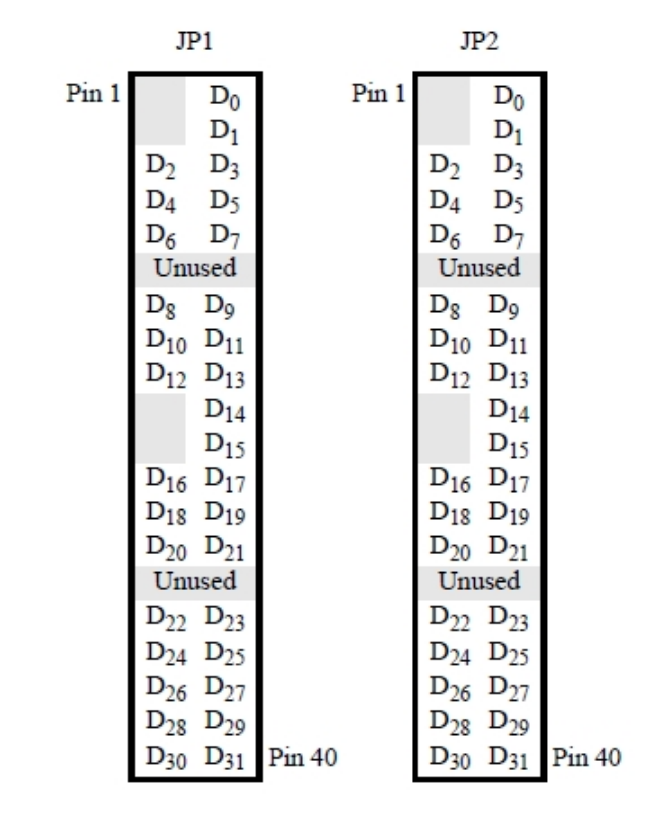
\includegraphics[width=0.8\linewidth]{img/image_2022-10-06-13-47-12.png}
	\caption{GPIO pinout}
\end{figure}


Two exercises we will cover include building a thermostat with the GPIO pins and building a keyboard.



\begin{listing}[H]
\begin{minted}{gas}
;; configure all pins as outputs
addi r8, r0, 0xFFFFFFFF
movia r9, 0xFF200064
stwio r8, 0(r9)

;; configure pins D0-D3 as outputs, D4-D31 as inputs
addi r8, r0, 0x0000000F
movia r9, 0xFF200064
stwio r8, 0(r9)
\end{minted}
\end{listing}

\marginnote{A write to an input pin will be silently ignored.}



Given that $ D_0 $ is connected to the thermostat's output and $ D_3 $ is connected to the heat fan motor,


\begin{listing}[H]
\begin{minted}{gas}
PIT1_BASE equ, 0xFF200060
PIT1_DR_OFFSET equ, 0x0
PIT1_DIR_OFFSET equ, 0x4

	.text
heat:
	movia r9, PIT1_BASE
	addi r8, r0, 8
	stwio PIT1_DIR_OFFSET(r9) ;; configure all pins but d3 as inputs (0x00000008)
	stwio r0, PIT1_DR_OFFSET(r9) ;; turn off the motor
fever:
	ldwio r8, PIT1_DR_OFFSET(r9) ;; read all pins
	andi r8, r8, 0x1 ;; mask off all but d0
	beq r8, r0, fanon ;; turn fan on because it's cold (d0 == 9)
fanoff:
	stwio r0, PIT1_DR_OFFSET(r9) ;; turn off the motor
	br fever
fanon:
	addi r8, 8
	stwio r8, PIT1_DR_OFFSET(r9) ;; turn on the motor
	br fever
\end{minted}
\end{listing}
\marginnote{In the lecture notes he uses 0x00000004 but I think that's a typo.}

Something similar can be implemented in \texttt{c} 

\begin{listing}[H]
\begin{minted}{c}

#define DR ((unsigned int* ) 0xFF200060)
#define DIR ((unsigned int* ) 0xFF200064)

void heat(void)
{
	unsigned int t;
	*DIR = 0x8;
	*DR = 0x0;
	while (1)
	{
		t = *DR;
		if (t & 0x1)
			*DR = 0x0;
		else
			*DR = 0x8;
	}
}
\end{minted}
\end{listing}


A nicer way that this can be implemented is to use a struct to represent the PIT


\begin{listing}[H]
\begin{minted}{c}

struct PIT_t {
	unsigned int DR;
	unsigned int DIR;
};

struct PIT_t *pitp = (struct PIT_t *) 0xFF200060;

void heat(void)
{
	unsigned int t;
	pitp->DIR = 0x8;
	pitp->DR = 0x0;
	while (1)
	{
		t = pitp->DR;
		if (t & 0x1)
			pitp->DR = 0x0;
		else
			pitp->DR = 0x8;
	}
}
\end{minted}
\end{listing}

This chunk of code exploits the fact that the DR element appears first and is immediately followed by DIR. This allows us to elegantly map the fields of the struct to the actual memory layout (line 7)

Another example let's consider debouncing the metal switch used inside the thermostat. Whenever metal contacts are used there is a short period of time where the switch will rapidly change state. This may not be what the user intends and as such we'd like to debounce the values to make it more sane.
To avoid this we take a number of samples and assume that the value read is 1 only if the number of samples that was 1 is greater than $ \frac{N}{2} $ 



\begin{listing}[H]
\begin{minted}{gas}
PIT1_BASE equ, 0xFF200060
PIT1_DR_OFFSET equ, 0x0
PIT1_DIR_OFFSET equ, 0x4

	.text
heat:
	movia r9, PIT1_BASE
	addi r8, r0, 8
	stwio PIT1_DIR_OFFSET(r9) ;; configure all pins but d3 as inputs (0x00000008)
	stwio r0, PIT1_DR_OFFSET(r9) ;; turn off the motor

fever:
	addi r10, r0, 1000 ;; take 1000 samples
	add r11, r0, r0 ;; count of samples that are 1

sampling:
	ldwio r8, PIT1_DR_OFFSET(r9) ;; read all pins
	andi r8, 0x1 ;; mask out r0 (thermostat)
	add r11, r11, r8 ;; increment count if r8 is 1
	subi r10, r10, 1 ;; decrement sample count
	bne r10, r0, sampling ;; loop if we still have samples to take

	addi r10, r10, 500 ;; check if we have more than 500 samples that are 1
	bgt r11, r10, fanon

fanoff:
	stwio r0, PIT1_DR_OFFSET(r9) ;; turn off the motor
	br fever

fanon:
	addi r8, 8
	stwio r8, PIT1_DR_OFFSET(r9) ;; turn on the motor
	br fever
\end{minted}
\end{listing}


\subsubsection{The PIT implementation}

This example is a PIT with 8 connections with $ DR $ at \texttt{0xFF1110}  and $ DIR $ at \texttt{0xFF1114}. A 32 bit PIT should follow.


At a physical level the PIT presents the following signals


\begin{enumerate}
	\item Data: 8 wires that supply the value to be written to or read from the PIT
	\item DIR write signal: when this is 1 the value in the data wires is written to the DIR
	\item DR write signal: when this is 1 the value in the data wires is written to the DR
	\item DR read signal: when this is 1 the data signals are placed into output mode and take on values that currently appear on external port connections
	\item External port: 8 wires that connect to the external world
\end{enumerate}


\begin{figure}[H]
	\centering
	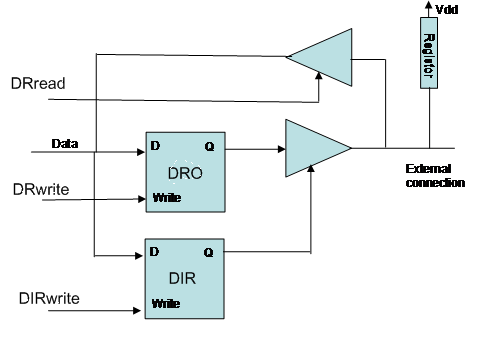
\includegraphics[width=0.8\linewidth]{img/image_2022-10-16-00-30-46.png}
	\caption{One PIT bit}
\end{figure}

The DRO and DIR boxes are latches whose values change using the Data and Write signals. The triangle looking things are \href{https://en.wikipedia.org/wiki/Three-state_logic}{tri-state buffers}.

\begin{itemize}
	\item DIR = 1 -> tri-state latch is closed -> passes value of DRO to external connection
	\item DIR = 0 -> tri-state latch is open -> external source determines value on the connection
		\begin{itemize}
			\item resistor helps drive high voltage from external source
		\end{itemize}
	\item DRread = 1 -> opens upper tristate buffer, puts external value into Data line
\end{itemize}

Eight of these can then be chained together to form a 8 bit PIT.


\subsubsection{Memory}

Our memory needs to meet these requirements

\begin{enumerate}
	\item Load/store operations
	\item Byte, halfword, or word types
	\item Addr of 32 bits
	\item data value of at most 32 bits for read/write values
	\item A do-nothing signal
\end{enumerate}

1) can be implemented with a signle read-write signal. 2)) can be done with 2 signals. Let's use 00 for byte, 01 for half-word, and 11 for long-word. 10 is not used.
3) and 4) need 32 signals each, and 5) requires a master-enable signal. This is useful to prevent the memory from taking on transient values.


Now comes the task of connecting the PIT to the memory interface.
First we connect the PIT data lines to the lower 8 bits of the memory interface. So DIR, DRO, DRI can be accessed via load/store operations


\begin{figure}[H]
	\centering
	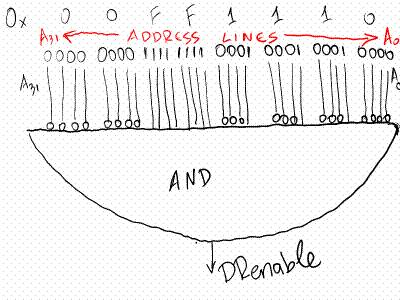
\includegraphics[width=0.8\linewidth]{img/image_2022-10-16-00-55-19.png}
	\caption{We'll also need to check if the address being accessed is the address of the PIT. The easiest way to do this is to just use an AND across the address lines and pass that signal to DREnable}
\end{figure}


DRenable can now be combined with R/W to form a single signal that generates the DRread and DRwrite signals


\begin{figure}[H]
	\centering
	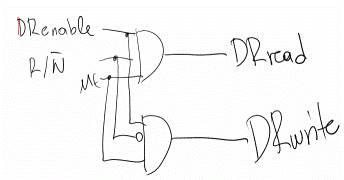
\includegraphics[width=0.8\linewidth]{img/image_2022-10-16-00-57-58.png}
\end{figure}

Something similar can be done for DIRwrite.

\begin{figure}[H]
	\centering
	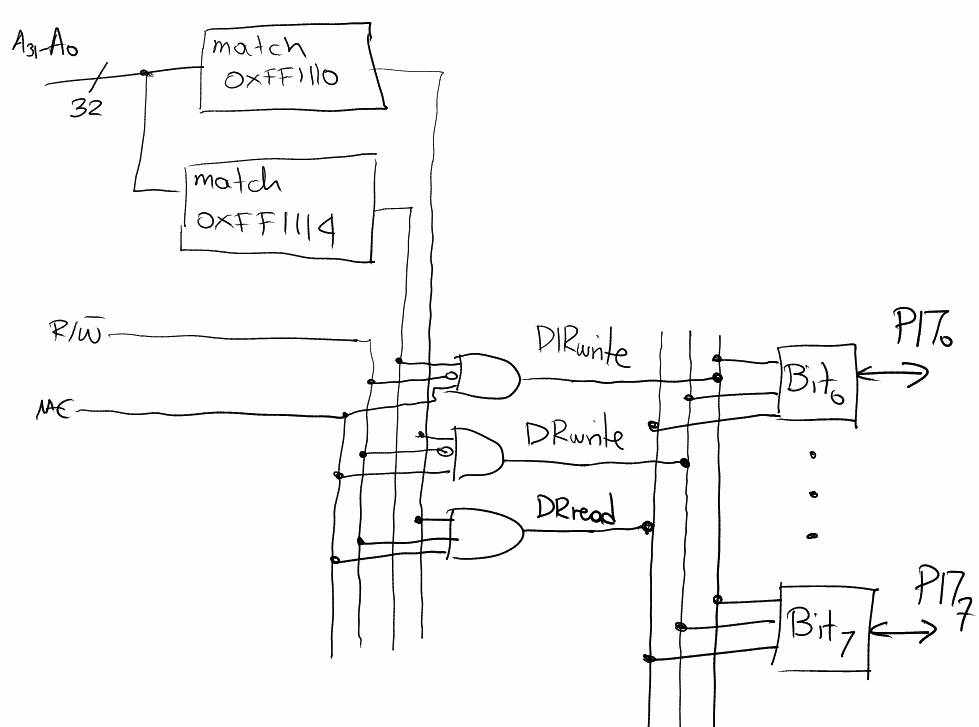
\includegraphics[width=0.8\linewidth]{img/image_2022-10-16-00-58-42.png}
	\caption{The complete design}
\end{figure}


\subsection{Lecture 12: UART}

The (JTAG) UART device is a UART implemented over the JTAG interface, which for the NIOSII is implemented over USB. 
UART stands for Universal Asynchronous Receiver Transmitter. It is a communication protocol which allows for non-instantaneous communication between two devices.


\begin{itemize}
	\item Starts at address \texttt{0xFF201000}
	\item Receiver Register RR at an offset of 0
	\item Transmitter Register at an offset of 0 (same as RR)
	\item Control and status register, CSR at an offset of 4
\end{itemize}

\begin{figure}[H]
	\centering
	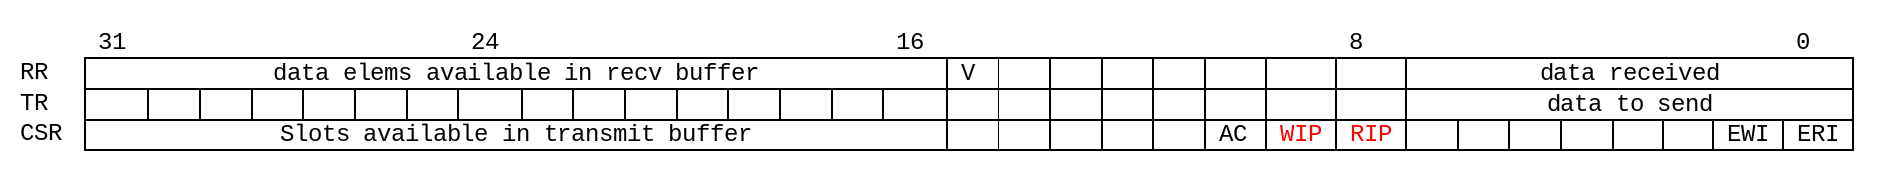
\includegraphics[width=0.8\linewidth]{img/image_2022-10-16-01-58-27.png}
	\caption{Register format}
\end{figure}

There are two transactions that can be asked of the UART: (1) send a character and (2) receive a character.
They are implemented by placing bits into the data to send/receive into the transmitter/receiver register.
However, in real life communication is more difficult than just that; sending characters takes considerably longer than the CPU's speed so we must be able to wait while the UART is sending a character before an attempt to send another one is made. Also, we should only read a character from the RR only if one has been received from the external source. This reading may also need to be buffered due to the variable nature of RR receive speed.


\textbf{sending a character}  

Here's a subroutine for sending the character in \texttt{r4}. 


\begin{listing}[H]
\begin{minted}{gas}
.equ JTAG_UART_BASE, 0xFF201000
.equ JTAG_UART_RR, 0
.equ JTAG_UART_TR, 0
.equ JTAG_UART_CSR, 4

	.text
putchar:
	movia r8, JTAG_UART_BASE
wait:
	ldwio r2, JTAG_UART_CSR(r8) # read csr
	srli r2, r2, 16 # keep only upper 16 (shift right logical immediate)
	;; The csr's bits 16-31 contains a number which
	;; is the number of slots in the queue avaliable 
	;; to accept requests. If the number is 0, then
	;; the queue is full and we must wait.
	beq r2, r0, wait # wait until upper 16 bits are nonzero

	stwio r4, JTAG_UART_TR(r8) # place it into the FIFIO
	ret
wait:



\end{minted}
\end{listing}


\textbf{receiving a character}

To receive a character we must wait until a character is received. This information is in RR

\begin{itemize}
	\item 0-7 contain the character, if one has been received
	\item 15 is 1 if a character has been received. If it is 0, then no character has been received and 0-7 are meaningless
	\item 31-16 contain additional information e.g. number of additional characters received and are waiting in the incoming queue.
\end{itemize}


\begin{listing}[H]
\begin{minted}{gas}
.equ JTAG_UART_BASE, 0xFF201000
.equ JTAG_UART_RR, 0
.equ JTAG_UART_TR, 0
.equ JTAG_UART_CSR, 4

	.text
getchar:
	movia r8, JTAG_UART_BASE

wait:
	ldwio r2, JTAG_UART_RR(r8) ;; read RR in r2
	andi r10, r2, 0x8000 ;; extract bit 15
	beq r10, r0, wait ;; wait until bit 15 is 1
	andi r2, r2, 0xff ;; keep only character (bit 0-7) in r2
	ret



\end{minted}
\end{listing}

\marginnote{Both of these subroutines busy waits are used. This is slow and inefficient. A better way is to use interrupts, which will be covered in a later lecture}



\begin{listing}[H]
\begin{minted}{gas}
;; An echo routine
.equ JTAG_UART_BASE, 0xFF201000
.equ JTAG_UART_RR, 0
.equ JTAG_UART_TR, 0
.equ JTAG_UART_CSR, 4

  .text
echo:
  movia r8, JTAG_UART_BASE
waitr:
  ldwio r2, JTAG_UART_RR(r8)    # read RR in r2
	# extract bit 15 in register r10 / keep a copy of r9 since it contains the character if any
  andi  r9, r2, 0x8000          
	# if bit 15 was zero, there was no character, keep waiting/trying
  beq   r9, r0, waitr           
	# a character was received, copy the lower 8 bits to r2 and return
  andi  r2, r2, 0xff            

waitt:
	# read CSR in r9
  ldwio r9, JTAG_UART_CSR(r8)   
	# keep only the upper 16 bits
  srli  r9, r9, 16              
	# as long as the upper 16 bits were zero keep trying
  beq   r9, r0, waitt           
	# place it in the FIFO
  stwio r2, JTAG_UART_TR(r8)    
	# life is interesting, keep doing what you do
  br    waitr                  
	# never reaches here, this is for show
  ret                           


\end{minted}
\end{listing}

At the communication link level the device represents the characters as a stream of bits. Each bit is communicated by setting the line to the corresponding voltage level for a pre-specified duration; this is the bit-cell shown.
\begin{definition}
	\textbf{baud rate} : number of bit cells within on second. For example 9600 baud means a bit time of $ \frac{1}{9600} = 104.16$ microseconds, so it would take 1.0416 milliseconds at least to send a full byte. Note that each byte has a start and stop bit so a byte takes 10 bit cells to transmit.
\end{definition}

Ideally the transmitter and receiver would use identical time references for the bit cells, which would make life easy because it would mean the receiver can simply just take a single sample at the center of each bit cell to reconstruct the byte. 
However, life is not so easy and real-life devices have phase differences. 
\begin{figure}[H]
	\centering
	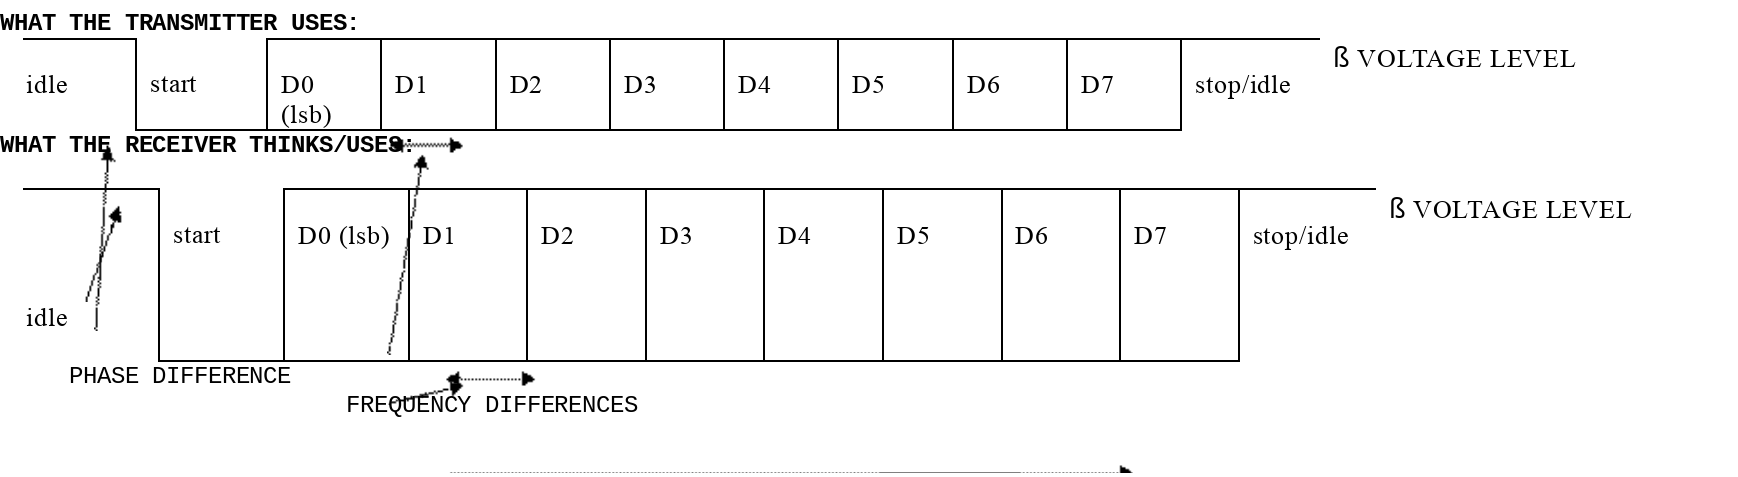
\includegraphics[width=0.8\linewidth]{img/image_2022-10-16-03-26-20.png}
	\caption{Phase differences}
\end{figure}

\sidenote{In practice there shoulnd't be a difference of more than 20\% between the stop bit and where the receiver things the stop bit is. This is because of RS-232C standard imposing a requirement imposing a maximum of 2\% difference between device baud rates, and the fact that there are start/stop bits which allow for the receiver to sync to sender time.}

The common solution for this problem is to use over-sampling, i.e. taking several samples to detect the 0->1 transition for the stop/idle to start bits, then making carefully chosen single samples to fall at the center of bit time. 
For a receiver that takes 16 samples per bit cell, generally the ith sample should be taken at $ (24 + i * 16) $  cycles, i.e. pass 16 samples to get past start bit and then another 8 to go to the middle of the first bit cell and so forth.

Even with these measures communication errors\sn{FRAME Errors} can still occur. Further reduction of errors can be achieved by using using an additional parity bit which can be used to detect single errors.



\begin{figure}[H]
	\centering
	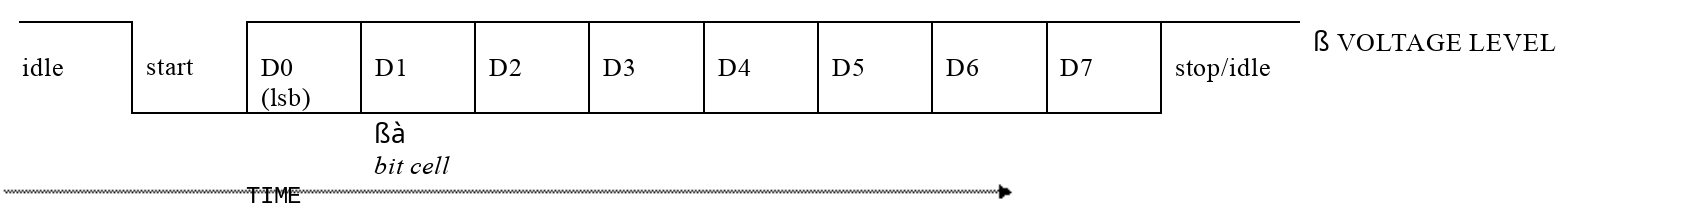
\includegraphics[width=0.8\linewidth]{img/image_2022-10-16-03-23-05.png}
\end{figure}

\subsection{Lecture 13: Interrupts \& UART}
In the previous lecture we used busy polling to communicate with the serial device, i.e. probing the status register until the desired condition was met.
Not only is this a wasteful use of device resources, it is also difficult to scale to multitasking scenarios.

At a high level, interrupts work as follows:


\begin{enumerate}
	\item The processor is executing instructions
	\item A device requests an interrupt
	\item The processor decides to grant that request, i.e. finishing current instruction and then inducing a call to a special interrupt handler routine
	\item Program flow is restored to previous instruction
\end{enumerate}


Therefore there are a few requirements that must be met for interrupts to work

\begin{enumerate}
	\item Devices must be able to request interrupts
	\item Must be able to signal to device that it's interrupt has been handled
	\item Must have a way to map interrupts to the correct interrupt handler
	\item Need to know where the interrupt handler lives in memory
	\item Must be able to save and restore state affected by an interrupt call
\end{enumerate}

Requirements 1 and 2 are handled by having two directed wires between the CPI and the device through which request and response `handshake's can be implemented. The NIOS II provides 32 interrupt request wires IRQ0 to IRQ31, and notifying a device is done in software i.e. writing to a specific location in memory. Exact process is device-specific.
Requirements 3 and 4 i.e. inducing an interrupt handler. One way that this can be done is to have a subroutine at a hard-coded address for all interrupts which then queries which device requested the interrupt and then inducing the call to the appropriate handler. This is generally implemented as some sort of lookup table. The NIOS II implements this by having all interrupt requests start executing code at \texttt{0x00000020}; the \texttt{.section exceptions, "ax"} directive can be used to assign code to that part of memory. That code must interrograte all devices to figure out which devices are requesting interrupts and then fire off the appropriate ISRs.
Requirement 5 can be met by just pushing everything relevant onto the stack.



\begin{definition}

	\begin{itemize}
		\item \textbf{ctl0}: Master interrupt enable switch. Bit 0 is 1 means interrupts will be serviced; they will be ignored otherwise.  
		\item \textbf{ctl1}: Preserves current state of ctl0 upon accepting an interrupt
		\item \textbf{ctl3}: Enable/disable specific IRQ lines. Interrupts are accepted for IRQ$i$ if bit $ i $ of ctl3 is 1 and bit 0 of ctl0 is 1
	\end{itemize}

	Reading and writing from control registers is done through two specialized instructions; \texttt{rdctl ctrlx, ry}: reads value of a control register ctrlx and stores in ry, and \texttt{wrctl ctrlx, ry} which writes the value of ry into ctrlx.
	Also, \texttt{r29} also participates by storing the PC of the instruction following that of the interrupt and commonly is aliased to be \texttt{ea}, or exception address.

\end{definition}

The more detailed sequences is therefore as follows

\begin{itemize}
	\item Device assert an IRQ line to request an interrupt
	\item Processor finishes current instruction
	\item Processor saves the current interrupt enable bit (storing ctl0 into ctl1), then disables ctl0 to disable further interrupts
	\item Set $ ea = PC + 4 $; the PC immediately following the instruction that had just been executed
	\item Set $ PC = 0x20 $ so that execution continues in interrupt handler
	\item Handler terminates with \texttt{eret} which will restore ctl0 from ctl1 and PC from ea
\end{itemize}


\subsection{Lecture 14: Timer}


In lieu of lecture notes here is a big chunk of code which uses the NIOSII timer device to wait a second.


\begin{listing}[H]
\begin{minted}{gas}
.equ  TIMER0_BASE,      0xFF202000
.equ  TIMER0_STATUS,    0
.equ  TIMER0_CONTROL,   4
.equ  TIMER0_PERIODL,   8
.equ  TIMER0_PERIODH,   12
.equ  TIMER0_SNAPL,     16
.equ  TIMER0_SNAPH,     20
.equ  TICKSPERSEC,      500000000
      .text
waitasec:
      movia r8, TIMER0_BASE
      addi  r9, r0, 0x8                   ;; stop the counter
      stwio r9, TIMER0_CONTROL(r8)
 
      ;; Set the period registers to 50M
      addi  r9, r0, %lo (TICKSPERSEC)
      stwio r9, TIMER0_PERIODL(r8)
      addi  r9, r0, %hi(TICKSPERSEC)
      stwio r9, TIMER0_PERIODH(r8)
 
;; tell the counter to start over automatically and start counting
      addi  r9, r0, 0x6                   ;; 0x6 = 0110 so we write 1 to START and to CONT
      stwio r9, TIMER0_CONTROL(r8)
 
onesec:
      ldwio       r9, TIMER0_STATUS(r8)   ;; check if the TO bit of the status register is 1
      andi        r9, r9, 0x1
      beq         r9, r0, onesec
 
      addi        r9, r9, 0x0             ;; clear the TO bit
 
      stwio       r9, TIMER0_STATUS(r8)
 
      ;; decrement the number of remaining seconds and repeat until this becomes zero
      subi        r4, r4, 1
     
      bne         r4, r0, onesec         
 
      ;; stop the counter before exiting
 
      addi        r9, r9, 8        
      stwio       r9, TIMER0_CONTROL(r8)
      ret
           
;; And here’s a function that calls waitasec asking it to wait for 20 seconds:
      .text
      .global main

main:
      addi  r4, r0, 20
      call  waitasec
      ret

\end{minted}
\end{listing}

Checking the current value of the period registers cannot happen directly and instead must be done through snap registers.

\begin{listing}[H]
\begin{minted}{gas}
   movia r8, TIMER0_BASE        
   stwio r0, TIMER0_SNAPL(r7)  # Take a snapshot of the period registers
   ldwio r9, TIMER0_SNAPL(r7)  # Read snapshot bits 0..15
   ldwio r10, TIMER0_SNAPH(r7) # Read snapshot bits 16...31
   slli  r10, r10, 16          # Shift the upper bits to positions 16 through 31 in register r10
   or    r9, r9, r10           # Combine bits 0..15 and 16...31 into one register
\end{minted}
\end{listing}


\subsection{Lecture 15: Code Races}

Consider the following c code:

\begin{listing}[H]
\begin{minted}{c}
      int   cnt = 9;
interrupt:
            cnt++;
program:
            while (1) cnt--;
\end{minted}
\end{listing}

At the machine code level this can look like

\begin{listing}[H]
\begin{minted}{gas}
      .data
cnt:  .word 9
      .section .exceptions, “ax”
iHdlr:     
H1:         ldw         r9, 0(r8)
H2:         addi        r9, r9, 1  
H3:         stw         r9, 0(r8)
            eret
      .text
main:
            movia       r8, cnt
            movi        r9, 1
            wrctl       ctl0, r1
wait:      
I1:         ldw         r11, 0(r8)
I2:         addi        r11, r11, -1
I3:         stw         r11, 0(r8)
            br          wait
\end{minted}
\end{listing}


We can possibly observe the sequence $ 10, 11, 10, 9$, and so forth because of a \textit{race} between the interrupt and the while loop.
This is because NIOS II does not implement atomic operations, therefore the same value can be loaded a register for two operations that change it without coordinating between the two programs, and therefore cause undesirable behaviour.
Other architectures may implement atomic operations, which are operations that cannot be by another instruction (usually at the expense of performance).

\subsubsection{Buffer Overflow Stack Attacks}

Consider the following \texttt{c} method which takes a \texttt{char*} input over the network


\begin{listing}[H]
\begin{minted}{c}
void packet_parse_string(char* packet){
	char buffer[100];
	// some code
	// copy packet (null-terminated string) into buffer
	while (packet[i]){
		buff[j++] = packet[i++];
	}
	// some other code
}
\end{minted}
\end{listing}

One may immediately notice that there is no check to see if the packet is larger than 100 bytes, and therefore the buffer may overflow.
Though this may seem like an innocuous invalid write, this function can be exploited to run arbitrary code.
From this course we know that when returning it will try to restore \texttt{RA} from the stack, perform \texttt{RET}, and start executing code from \texttt{PC=RA}.
This means that if the malicious caller can identify where the top of the stack was when calling, they may change the value of \texttt{RA} via the buffer overflow to the address of \texttt{buffer} and therefore execute arbitrary code that they sent inside of \texttt{packet}.


Ways to defend against such attacks include writing non-sloppy code or forbidding execution of code on the stack\mn{though there are valid reasons for doing this at times, i.e. JIT compilation.}


\subsection{Lecture 16: Emulating instructions in software}

Interrupts can be used for more than just communicating with I/O devices, i.e. for detecting erroneous conditions during execution, misaligned memory access, or OS calls.
They can also be used to emulate an instruction in software.

For example, on the NIOSII there is a \texttt{mulxuu rC, rA, rB} instruction to multiply two 32 bit registers and then store the upper 32 bits of the result into a rC.
Some NIOSII implementations may include a hardware unit which implements this instruction, but others may rely on emulation to execute this instruction instead.
Likewise, the 80386 processor does not have a hardware unit to implement floating point instructions (but one could do them in hardware with the 80387 co-processor). If one did not have the 80387 they can use interrupts to emulate the instruction in software instead (though slower)




\begin{figure}[H]
	\centering
	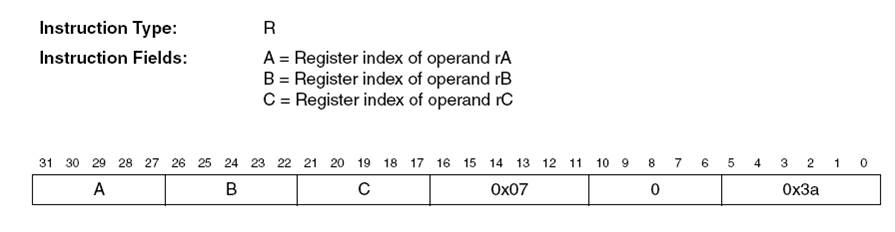
\includegraphics[width=0.8\linewidth]{img/image_2022-11-03-14-27-58.png}
	\caption{Encoding of the \texttt{mulxuu} instruction}
\end{figure}

Bits 31-27, 26-22, 21-17 encodes the source and destination registers. 16-11 contains 0x7, 10-6 the value 0, and 5-0 the value 0x31. So TLDR bit 16 is 0 and the lower 16 bits 0x383a.



\begin{figure}[H]
	\centering
	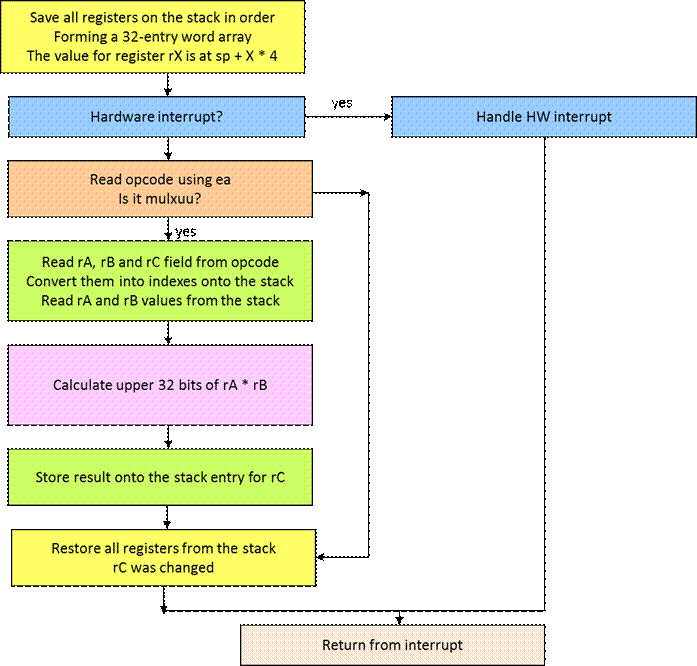
\includegraphics[width=0.8\linewidth]{img/image_2022-11-03-14-30-03.png}
	\caption{Interrupt handler flowchart}
\end{figure}



This chunk of code implements the first item in the flow chart, saving all the registers onto the stack. Note the commented \texttt{rdctl} checking for software interrupts

\begin{listing}[H]
\begin{minted}{gas}
      .section exceptions
 
      ; tell the assembler to not introduce any additional instructions overwriting registers
      .set nobreak
      .set noat
 
handler:                                                                       
        ;;;;;;;;;;;;;;;;;;;;;;;;;;;;;;;;;;;;;;;;;;;
        ; store all registers on the stack
        ; forming an array of words
        ; the value for register X is at sp+X*4 where X a number 0...32
        ;;;;;;;;;;;;;;;;;;;;;;;;;;;;;;;;;;;;;;;;;;;
        ; save all registers on the stack
        subi  sp, sp, 32 * 4
        stw r0,0(sp)
        stw r1,4(sp)
        stw r2,8(sp)
        stw r3,12(sp)
        stw r4,16(sp)
        stw r5,20(sp)
        stw r6,24(sp)
        stw r7,28(sp)
        stw r8,32(sp)
        stw r9,36(sp)
        stw r10,40(sp)
        stw r11,44(sp)
        stw r12,48(sp)
        stw r13,52(sp)
        stw r14,56(sp)
        stw r15,60(sp)
        stw r16,64(sp)
        stw r17,68(sp)
        stw r18,72(sp)
        stw r19,76(sp)
        stw r20,80(sp)
        stw r21,84(sp)
        stw r22,88(sp)
        stw r23,92(sp)
        stw r24,96(sp)
        stw r25,100(sp)
        stw r26,104(sp)
        stw r27,108(sp)
        stw r28,112(sp)
        stw r29,116(sp)
        stw r30,120(sp)
        stw r31,124(sp)
      rdctl et, ctl4                ; Check that interrupt was caused by      software
      beq et, r0, software          ; if not, it's a hardware interrupt ignore
     
      HANDLE HARDWARE INTERRUPTS HERE
 
      br  iEpilogue

\end{minted}
\end{listing}

The software interrupt handler checks the opcode in order pass execution to the appropriate subroutine. For \texttt{mulxuu} this is just comparing the lower 16 bits of \texttt{ea} with \texttt{0x383a}

\begin{listing}[H]
\begin{minted}{gas}
      ;;;;;;;;;;;;;;;;;;;;;;;;;;;;;;;;;;;;;;;;;;;;;;;;;;;;;
      ; read the instruction opcode to test whether it is a mulxuu
      ; ea points to the instruction
      ;;;;;;;;;;;;;;;;;;;;;;;;;;;;;;;;;;;;;;;;;;;;;;;;;;;;;
software:
      ldw   r9, -4(ea) ;; lecture notes uses stw but this should be ldw
      add   r10, r9, r0 ; keep a copy of the opcode
      andi  r9, r9, 0xffff    ; keep just the lower 16 bits
      cmpeqi      r11, r9, 0x383a
      beq   r11, r0, notmulxuu
      srli  r10, r10, 16      ; shift the upper 16 bits into the lower 16
      andi  r11, r10, 0x1     ; test bit 0 which used to be bit 17
      bne   r11, r0, notmulxuu ; if not zero this is not mulxuu

\end{minted}
\end{listing}


If we get to the \texttt{mulxuu} handler we need to load the registers from the stack


\begin{listing}[H]
\begin{minted}{gas}
      ;;;;;;;;;;;;;;;;;;;;;;;;;;;;;;;;;;;;;;;;;;;;;;;;;;;;;
      ; Operand index calculations
      ;;;;;;;;;;;;;;;;;;;;;;;;;;;;;;;;;;;;;;;;;;;;;;;;;;;;;
ismulxuu:
      ; now calculate indexes into the stack for accessing
      ; the input and output operands
      ; treat the stack as a 32-entry array of words
      ; we extract the 5 bit field for each operand
      ; multiply by four because each entry is four bytes
      ; and add the stack point which is the base of the array
      ;;;;;;;;;;;;;;;;;;;;;;;;;;;;;;;;;;;;;;;;;;;;;;;;;;;;;
      srli  r10,r10,1   ; keep just the upper 15 bits of the opcode
      ; rC
      andi  r11, r10, 0x1f    ; these are the 5 bits indicating rC the destination register
      slli  r11, r11, 2 ; multiply by 4
      add   r11, r11, sp      ; add the base of the array
      ; rB
      srli  r10, r10, 5
      andi  r12, r10, 0x1f ; keep the bits for rB
      slli  r12, r12, 2 ; multiply by 4
      add   r12, r12, sp      ; add the base of the array
      ; rA
      srli  r10, r10, 5
      andi  r13, r10, 0x1f ; keep the bits for rA
      slli  r13, r13, 2 ; multiply by 4
      add   r13, r13, sp      ; add the base of the array

\end{minted}
\end{listing}


...and then multiply the two registers and store the upper 32 bits into the destination register.

\begin{listing}[H]
\begin{minted}{gas}
 
      ;;;;;;;;;;;;;;;;;;;;;;;;;;;;;;;;;;;;;;;;;;;;;;;;;;;;;
      ; Access input registers
      ;;;;;;;;;;;;;;;;;;;;;;;;;;;;;;;;;;;;;;;;;;;;;;;;;;;;;
      ; at this point:
      ; r11 points to the entry for rC
      ; r12 points to the entry for rB
      ; r13 points to the entry for rA
      ; read rA and rB into r9 and r10 respectively
      ;;;;;;;;;;;;;;;;;;;;;;;;;;;;;;;;;;;;;;;;;;;;;;;;;;;;;
      stw r9, 0(r13)
      stw r10, 0(r12)
 
      ;;;;;;;;;;;;;;;;;;;;;;;;;;;;;;;;;;;;;;;;;;;;;;;;;;;;;
      ; Multiplication : No need to understand how this works
      ; end result is in r10
      ; I haven’t tested it much :(
      ;;;;;;;;;;;;;;;;;;;;;;;;;;;;;;;;;;;;;;;;;;;;;;;;;;;;;
      srli  r4, r9, 16  ; a = (v1 >> 16) & 0xffff;
      andi  r5, r9, 0xffff    ; b = v1 & 0xffff;
      srli  r6, r10, 16 ; c = (v2 >> 16) & 0xffff
      andi  r7, r10, 0xffff   ; d = v2 & 0xffff;
 
      mul   r9, r5, r7  ; LO = b * d;
      srli  r9, r9, 16  ; y = ((LO >> 16) & 0xffff)
      mul   r10, r4, r7 ; x= a * d
      mul   r12, r5, r6 ; x1 = c * b
      add   r10, r10, r12     ; x = x + x1
      add   r9, r9, r10 ; y = y + x
      srli  r9, r9, 16  ; y = (y >> 16) & 0xffff
      mul   r10, r4, r6 ; HI = a * c
      add   r10, r10, r9      ; HI = HI + y
 
      ;;;;;;;;;;;;;;;;;;;;;;;;;;;;;;;;;;;;;;;;;;;;;;;;;;;;;
      ; write result onto the corresponding stack entry
      ;;;;;;;;;;;;;;;;;;;;;;;;;;;;;;;;;;;;;;;;;;;;;;;;;;;;;
      ; store the result to the stack
      stw r10, 0(r11)
 
      ; declare this instruction as executed
      addi  ea, ea, 4


\end{minted}
\end{listing}

And clean up!

\begin{listing}[H]
\begin{minted}{gas}



 
iEpilogue:
notmulxuu:
        ;;;;;;;;;;;;;;;;;;;;;;;;;;;;;;;;;;;;;;;;;;;
        ; restore all registers from the stack
        ; one value has been changed
        ;;;;;;;;;;;;;;;;;;;;;;;;;;;;;;;;;;;;;;;;;;;
        stw r0,0(sp)
        stw r1,4(sp)
        stw r2,8(sp)
        stw r3,12(sp)
        stw r4,16(sp)
        stw r5,20(sp)
        stw r6,24(sp)
        stw r7,28(sp)
        stw r8,32(sp)
        stw r9,36(sp)
        stw r10,40(sp)
        stw r11,44(sp)
        stw r12,48(sp)
        stw r13,52(sp)
        stw r14,56(sp)
        stw r15,60(sp)
        stw r16,64(sp)
        stw r17,68(sp)
        stw r18,72(sp)
        stw r19,76(sp)
        stw r20,80(sp)
        stw r21,84(sp)
        stw r22,88(sp)
        stw r23,92(sp)
        stw r24,96(sp)
        stw r25,100(sp)
        stw r26,104(sp)
        stw r27,108(sp)
        stw r28,112(sp)
        stw r29,116(sp)
        stw r30,120(sp)
        stw r31,124(sp)
 
      ; restore the stack
      addi  sp, sp, 32 * 4
      br    idone
 
      ; for hardware interrupts re-execute instruction that was interrupted
eadec:
      subi  ea, ea, 4
idone:
      eret
\end{minted}
\end{listing}




A piece of code that uses the new instruction is therefore


\begin{listing}[H]
\begin{minted}{gas}
main:
	    movhi r9, 0xffff
      ori   r9, r9, 0xffff
      add   r10, r9, r0
      mulxuu r11, r9, r10
\end{minted}
\end{listing}




\subsection{Lecture 17: A single cycle processor}

For the purposes of this class we will consider a simple CPU capable of executing these 10 instructions (which are encoded as follows)

\begin{enumerate}
	\item \textbf{\texttt{load r1, r2}}
		\begin{listing}[H]
		\begin{minted}{text}
		TMP = MEM [R2]
		R1 = TMP
		PC = PC + 1
		\end{minted}
		\end{listing}

		\begin{figure}[H]
			\centering
			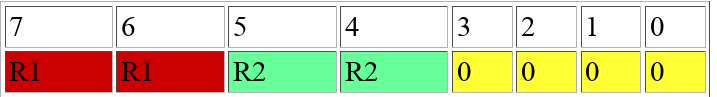
\includegraphics[width=0.8\linewidth]{img/image_2022-11-03-14-54-07.png}
		\end{figure}
		
	\item \textbf{\texttt{store r1, r2}}
		\begin{listing}[H]
		\begin{minted}{text}
     MEM [R2] = R1
		 PC = PC + 1
		\end{minted}
		\end{listing}
		\begin{figure}[H]
			\centering
			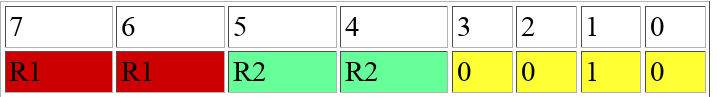
\includegraphics[width=0.8\linewidth]{img/image_2022-11-03-14-54-23.png}
		\end{figure}
	\item \textbf{\texttt{add r1, r2}}
		\begin{listing}[H]
		\begin{minted}{text}
     TMP = R1 + R2
     R1 = TMP
			IF (TMP == 0) ZERO = 1; ELSE ZERO = 0;
			IF (TMP < 0) NEGATIVE = 1; ELSE NEGATIVE = 0;
     PC = PC + 1
		\end{minted}
		\end{listing}
		\begin{figure}[H]
			\centering
			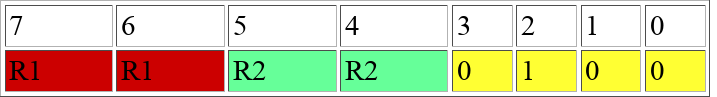
\includegraphics[width=0.8\linewidth]{img/image_2022-11-03-14-54-35.png}
		\end{figure}

	\item \textbf{\texttt{sub r1, r2}}
		\begin{listing}[H]
		\begin{minted}{text}
     TMP = R1 - R2
     R1 = TMP
		IF (TMP == 0) ZERO = 1; ELSE ZERO = 0;
		IF (TMP < 0) NEGATIVE = 1; ELSE NEGATIVE = 0;
		PC = PC + 1
		\end{minted}
		\end{listing}

		\begin{figure}[H]
			\centering
			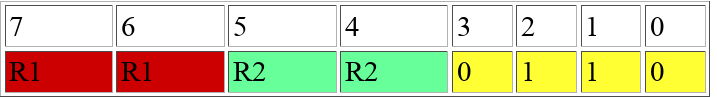
\includegraphics[width=0.8\linewidth]{img/image_2022-11-03-14-54-44.png}
		\end{figure}

	\item \textbf{\texttt{nand r1, r2}}
		\begin{listing}[H]
		\begin{minted}{text}
     TMP = R1 bitwise NAND R2
     R1 = TMP
		IF (TMP == 0) ZERO = 1; ELSE ZERO = 0;
		IF (TMP < 0) NEGATIVE = 1; ELSE NEGATIVE = 0;
		 PC = PC + 1
		\end{minted}
		\end{listing}

		\begin{figure}[H]
			\centering
			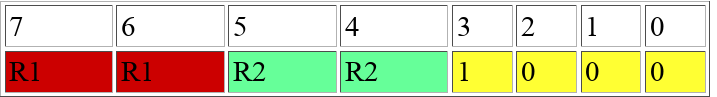
\includegraphics[width=0.8\linewidth]{img/image_2022-11-03-14-54-54.png}
		\end{figure}

	\item \textbf{\texttt{ori imm5}}
		\begin{listing}[H]
		\begin{minted}{text}
		TMP = K1 bitwise OR IMM5, where IMM5 is a 5 bit constant
		K1 = TMP
		IF (TMP == 0) ZERO = 1; ELSE ZERO = 0;
		IF (TMP < 0) NEGATIVE = 1; ELSE NEGATIVE = 0;
		PC = PC + 1
		\end{minted}
		\end{listing}

		\begin{figure}[H]
			\centering
			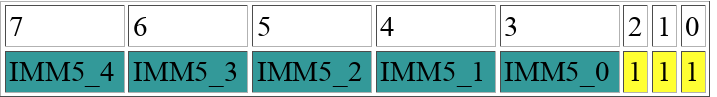
\includegraphics[width=0.8\linewidth]{img/image_2022-11-03-14-59-07.png}
		\end{figure}






	\item \textbf{\texttt{shift\{left, right\} r1, r2}}
		\begin{listing}[H]
		\begin{minted}{text}
     IF (L) THEN TMP = R1 << IMM2
            ELSE TMP = R1 >> IMM2
     R1 = TMP
IF (TMP == 0) ZERO = 1; ELSE ZERO = 0;
IF (TMP < 0) NEGATIVE = 1; ELSE NEGATIVE = 0;
PC = PC + 1
Alternative definition (equivalent to the previous one):
          IMM3 is a 3 bit immediate in the sign – magnitude representation, i.e., bit 2 = sign, value = bits 1 and 0
          IF (IMM3 > 0) THEN TMP = R1 << IMM3
                       ELSE TMP = R1 >> (-IMM3)
          R1 = TMP
IF (TMP == 0) ZERO = 1; ELSE ZERO = 0;
IF (TMP < 0) NEGATIVE = 1; ELSE NEGATIVE = 0;
PC = PC + 1
		\end{minted}
		\end{listing}

		\begin{figure}[H]
			\centering
			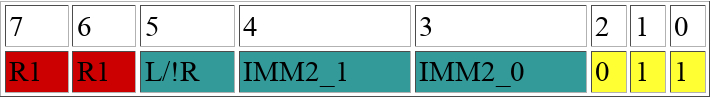
\includegraphics[width=0.8\linewidth]{img/image_2022-11-03-14-59-19.png}
		\end{figure}

	\item bz imm4
		\begin{listing}[H]
		\begin{minted}{text}
     where IMM4 is a 2’s complement 4-bit immediate
     IF (ZERO == 1) PC = PC + 1 + (SIGN-EXTEND8(IMM4))
     ELSE PC = PC + 1
		\end{minted}
		\end{listing}
		\begin{figure}[H]
			\centering
			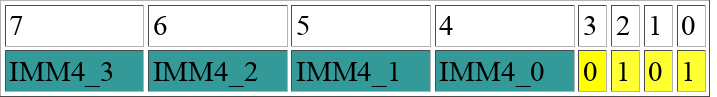
\includegraphics[width=0.8\linewidth]{img/image_2022-11-03-14-59-29.png}
		\end{figure}


	\item bnz imm4
		\begin{listing}[H]
		\begin{minted}{text}
     IMM4 as in BZ
     IF (ZERO == 0) PC = PC + 1 + (SIGN-EXTEND8(IMM4))
     ELSE PC = PC + 1
		\end{minted}
		\end{listing}
		\begin{figure}[H]
			\centering
			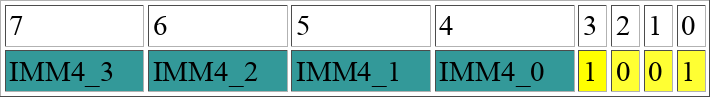
\includegraphics[width=0.8\linewidth]{img/image_2022-11-03-14-59-39.png}
		\end{figure}


	\item \textbf{\texttt{bpz imm4}}
		\begin{listing}[H]
		\begin{minted}{text}
     IMM4 as in BZ
     IF (NEGATIVE == 0) PC = PC + 1 + (SIGN-EXTEND8(IMM4))
     ELSE PC = PC + 1
		\end{minted}
		\end{listing}
		\begin{figure}[H]
			\centering
			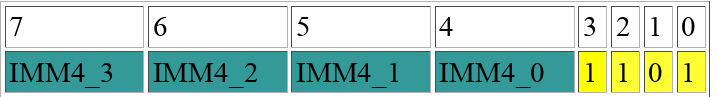
\includegraphics[width=0.8\linewidth]{img/image_2022-11-03-14-59-46.png}
		\end{figure}

\end{enumerate}


A CPU can be broken down into two units: the datapath and the control path. The data path is where all the data manipulation occurs; it should be capable of computing all results of the instruction execution.
The control path orchestrates signals sent to the data path (by means of a giant FSM).

\begin{figure}[H]
	\centering
	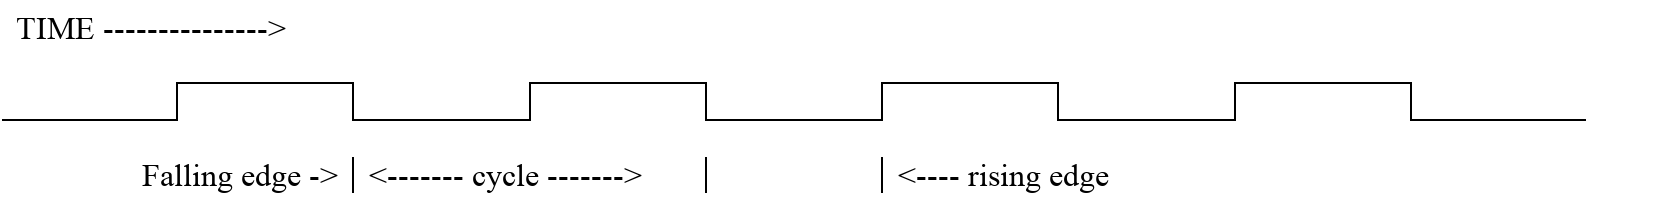
\includegraphics[width=0.8\linewidth]{img/image_2022-12-10-15-35-41.png}
	\caption{In the single-cycle processor each instruction will be executed entirely inside a single cycle. Code execution starts immediately after a falling edge and then all state changes will be complete right before the next falling edge.}
\end{figure}

CPU components include:

\begin{definition}
	Register
	\begin{figure}[H]
		\centering
		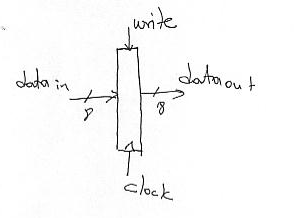
\includegraphics[width=0.8\linewidth]{img/image_2022-12-10-15-37-08.png}
		\caption{A collection of D flip-flops that can be read or written. Dataout gives values in the register, adding new values via datain. Write wire tells the register to latch onto the values in datain}
	\end{figure}
\end{definition}

\begin{definition}
	Mux
	\begin{figure}[H]
		\centering
		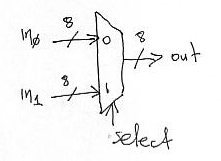
\includegraphics[width=0.8\linewidth]{img/image_2022-12-10-15-38-14.png}
		\caption{Multiplexes (Muxs) select a signal}
	\end{figure}
\end{definition}


\begin{definition}
	Register File

	\begin{figure}[H]
		\centering
		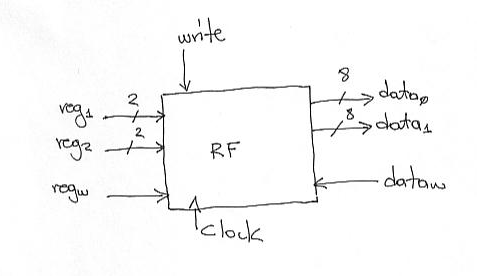
\includegraphics[width=0.8\linewidth]{img/image_2022-12-10-15-38-48.png}
		\caption{A register file contains a number of registers. Input signals to the register file cause it to output the data from the corresponding register to the data out lines. It also supports selecting and writing to a register by means of \texttt{regw} and \texttt{dataw}}. Note \texttt{write} signal as well.

		\begin{figure}[H]
			\centering
			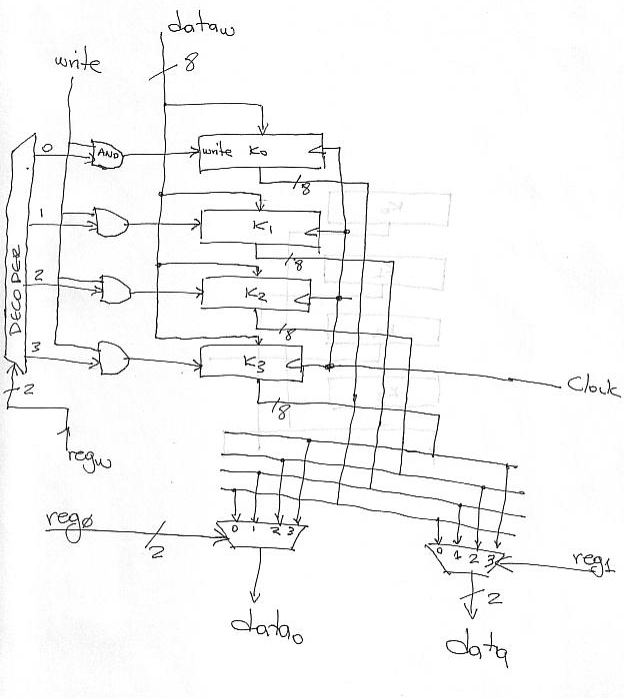
\includegraphics[width=0.8\linewidth]{img/image_2022-12-10-15-40-29.png}
			\caption{A register file implementation}
		\end{figure}
	\end{figure}
	
\end{definition}

\begin{definition}
	ALU
	\begin{figure}[H]
		\centering
		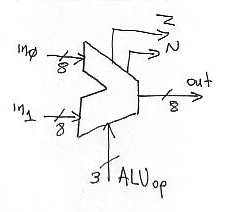
\includegraphics[width=0.8\linewidth]{img/image_2022-12-10-15-42-21.png}
		\caption{An ALU takes two inputs and then performs an operation as determined by the ALUOp signal. In this generalized ALU block we have $ Z, N $ signals which indicate if output values are zero or negative. Simpler ALUs can be used at times if things such as only addition is necessary}
	\end{figure}

	\begin{figure}[H]
		\centering
		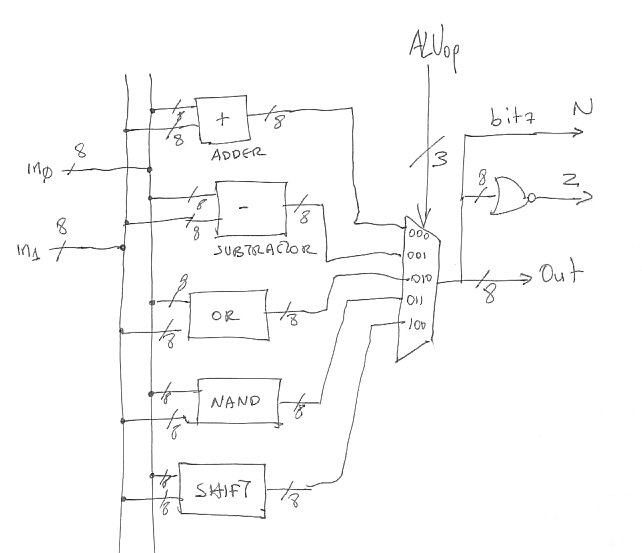
\includegraphics[width=0.8\linewidth]{img/image_2022-12-10-15-43-11.png}
		\caption{Possible impl}
	\end{figure}


	The and/sub boxes are fairly trivial, and so or OR/ANDs. Shift is a little more interesting
	\begin{figure}[H]
		\centering
		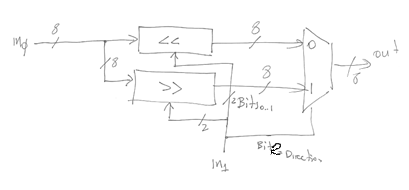
\includegraphics[width=0.8\linewidth]{img/image_2022-12-10-15-45-15.png}
		\caption{Shift is muxed on a shift left and a shift right}
	\end{figure}

	\begin{figure}[H]
		\centering
		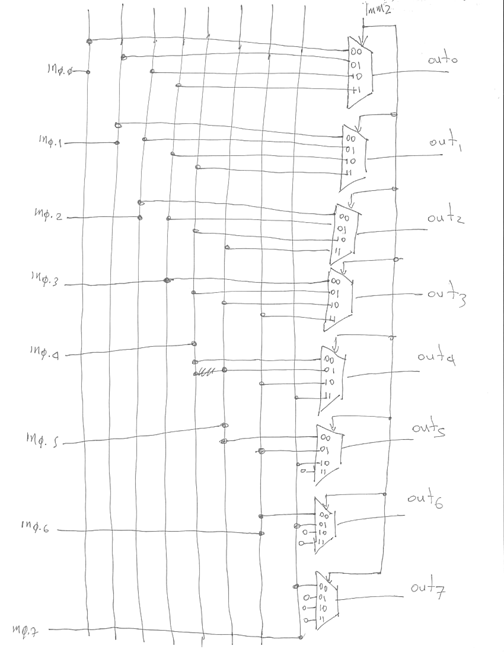
\includegraphics[width=0.8\linewidth]{img/image_2022-12-10-15-45-32.png}
		\caption{Shift left is a ton of muxes}
	\end{figure}

	\begin{figure}[H]
		\centering
		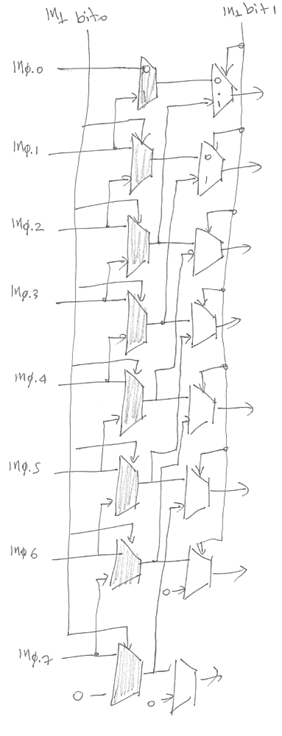
\includegraphics[width=0.8\linewidth]{img/image_2022-12-10-15-45-43.png}
		\caption{A shift by N is a series of shifts by 2. The barrel shifter takes advantage of this.}
	\end{figure}
\end{definition}

Most modern processors use unified instruction and data memories. For the single-cycle processor we will use the \textit{Harvard Architecture} which uses separate instruction and data memories.


\begin{figure}[H]
	\centering
	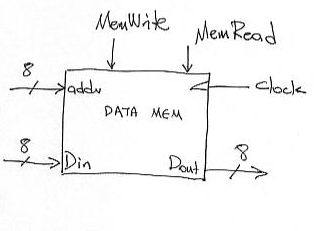
\includegraphics[width=0.8\linewidth]{img/image_2022-12-10-15-56-13.png}
	\caption{Memory}
\end{figure}

Data memory is capable of reading and writing (whereas instruction memory is read-only). Generally speaking it takes an address and depending on the value of MemWrite or MemRead it will either update the value at the address with \texttt{Din} or present the value at \texttt{Dout}



\begin{figure}[H]
	\centering
	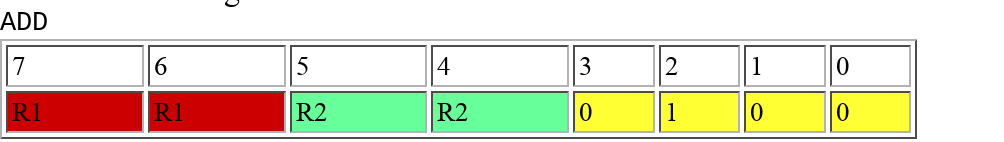
\includegraphics[width=0.8\linewidth]{img/image_2022-12-10-15-58-01.png}
	\caption{Recall: format of ADD instruction}
\end{figure}



\begin{figure}[H]
	\centering
	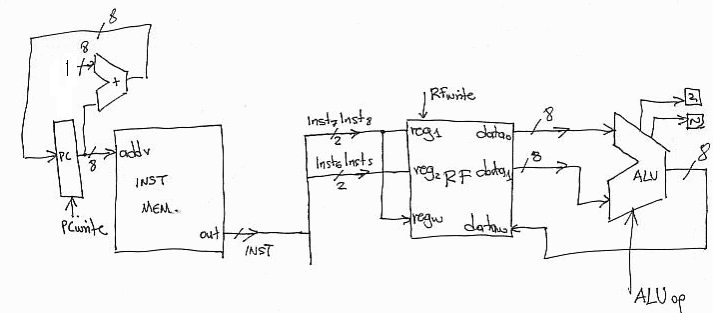
\includegraphics[width=0.8\linewidth]{img/image_2022-12-10-16-18-18.png}
	\caption{Datapath for ADD}
\end{figure}

Notice that bits 7 and 8 of the instruction are being piped directly into \texttt{reg1} and \texttt{regw} since our instruction definition gives \texttt{reg1 = reg1 + reg2}. The adder attached to the PC register is used to increment PC after each cycle.


\begin{figure}[H]
	\centering
	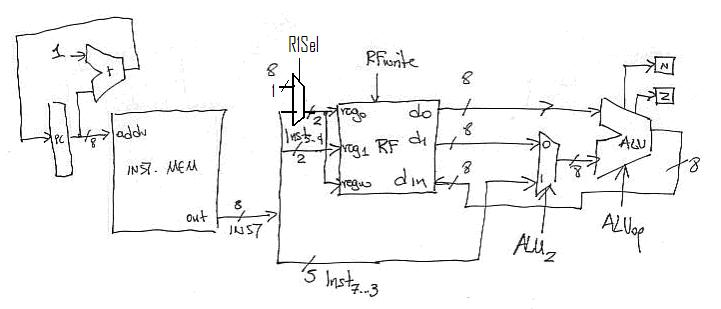
\includegraphics[width=0.8\linewidth]{img/image_2022-12-10-16-34-47.png}
	\caption{Augmented datapath to support ORI}
\end{figure}

ORI takes an immediate value from the instruction.




\subsection{Lecture 18: Modifying the single cycle processor}
\subsection{Lecture 19: Multi-cycle processor}


\texttt{ADD R1, R2}


\begin{enumerate}
	\item Read mem[PC] into IR.

\begin{figure}[H]
	\centering
	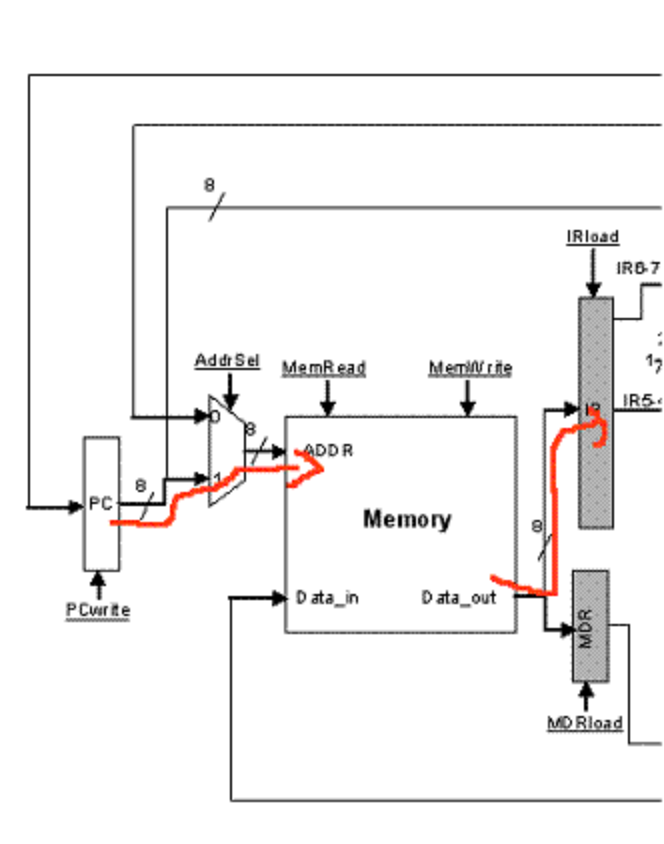
\includegraphics[width=0.8\linewidth]{img/image_2022-11-03-13-24-33.png}
	\caption{Cycle one for the ADD. This fetches the instruction by sending the address from PC register to MemRead and then storing the stored instruction into the Instruction Register IR}
\end{figure}

\item Decoding the instruction and reading from the register file


	\begin{figure}[H]
		\centering
		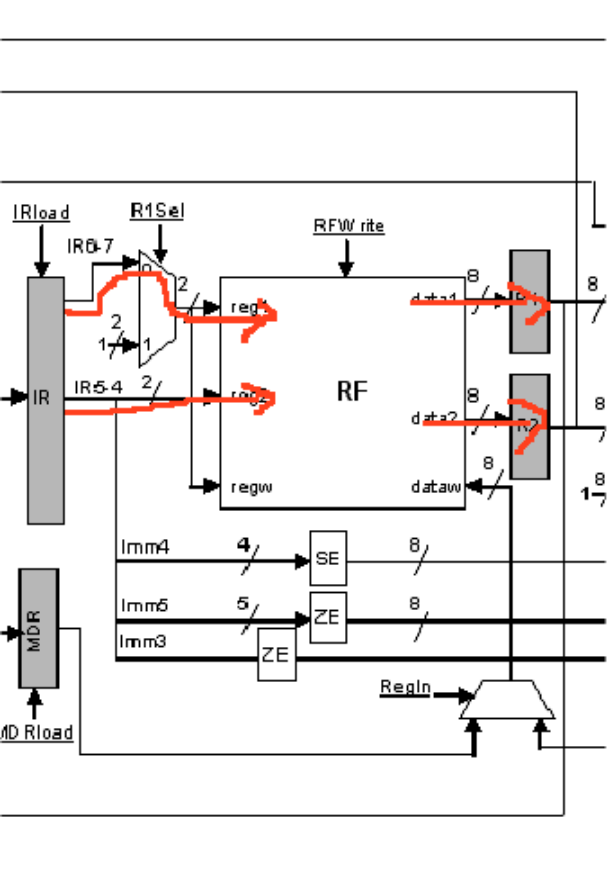
\includegraphics[width=0.8\linewidth]{img/image_2022-11-03-13-27-06.png}
		\caption{Control uses the instruction opcode to decide what happens during the next cycle. In this case, we read the two registers from the register file RF and then latch them into R1, R2}
	\end{figure}

\item R1 = RF[127, 6], R2 = RF[IR5, 4]


\item AluOut = R1 + R2, update Z \& N (Zero, Negative flags)
	This is done by muxing the latched values into the ALU (as well as the appropriate instruction as applicable) and then latching the ALU output and zero/negative flags. This step can be combined with the above step (discussed later).

\item RF[127, 6] = AluOut

\item Increment PC by 1.
	At this point the ALU is idle, so we can take a small detour and increment PC.



\end{enumerate}
By the end of this, this just needs to ensure that the programmer sees the desired behaviour; that the values have been added and the PC has been incremented.


What are some optimizations?

\begin{itemize}
	\item PC: reading at cycle 1, read at cycle 6. So we only need the current value at the beginning of cycles 1 and 6, so if we think about this we can probably speed things up by hoisting cycle 6 to cycle 1. So Cycle 1 can become PC = PC + 1 \marginnote{LHS happens at end of clock cycle, RHS happens during}. This way we can save a clock cycle. While this may sound good on paper, can it happen during actual execution? In this case nobody else is using the ALU during cycle 1, so this would only necessitate a change in control. This optimization is always ideal, all the time.
	\item Another optimization can happen during Cycle 2 and 3. It isn't certain that we can move Cycle 3 into Cycle 2; sometimes this will be helpful and sometimes it won't be helpful. But, it'll be helpful \textit{always} and it won't destroy any state. So we can \textit{speculate} that storing these results into the registers will \textit{probably} be useful and combine steps and 2. This gives us 
		\begin{enumerate}
			\item  PC = PC + 1
			\item  Decode \& Read from RF, R1 = RF[IR7, 6], R2 = RF[IR5, 4]
			\item  AluOut = R1 + R2, update Z \& N (Zero, Negative flags)
			\item  RF[IR7, 6] = AluOut
		\end{enumerate}
		\marginnote{There are situations where we speculate in a way that will destroy the state of the machine and then it turns that the speculation is not that helpful.}
\end{itemize}


\begin{blockquote}
	Note that cycle 1 and cycle 2 must be the exact same for all instructions -- this is because at that point we don't know what the instruction actually is. Only after instruction 2 do they change.
\end{blockquote}


\texttt{ORI imm5}

\begin{enumerate}
	\item Read mem[PC]
	\item Decode the instruction and read from the register file (R1, R2). We've read both but we only need one of them. But it doesn't hurt that we already have R2.
	\item R1 = RF[K1]
	\item ALUout = R1 OR imm5 (zero-extended)

		\begin{figure}[H]
			\centering
			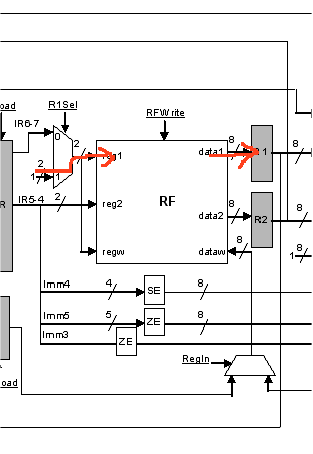
\includegraphics[width=0.8\linewidth]{img/image_2022-11-03-13-49-54.png}
			\caption{Note that imm5 is actually encoded into the instruction (see the control path)}
		\end{figure}
		\marginnote{We could've actually speculated another way to favor the ORI instruction to make it take 4 cycles instead. But statistically speaking the NAND, ADD, and SUB instructions end up being used a lot more often and therefore more useful to optimize for}
	\item RF[K1] = ALUout


\end{enumerate}


\texttt{LOAD}

\begin{figure}[H]
	\centering
	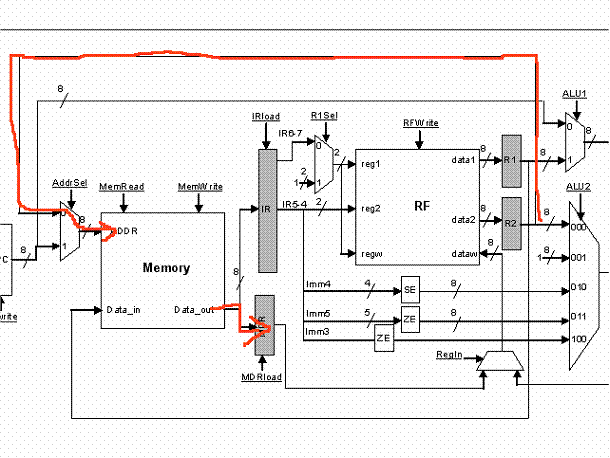
\includegraphics[width=0.8\linewidth]{img/image_2022-11-03-13-55-59.png}
	\caption{The \texttt{LOAD} instruction accesses memory during cycle 3 and then stores the returned value into MDR.}
\end{figure}

\begin{figure}[H]
	\centering
	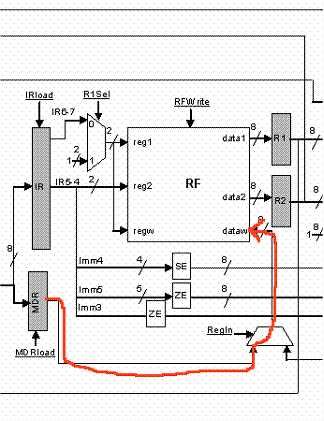
\includegraphics[width=0.8\linewidth]{img/image_2022-11-03-13-56-42.png}
	\caption{In cycle 4 the MDR value can be written to the register file.}
\end{figure}


\texttt{STORE}


\begin{enumerate}
	\item PC = PC+1; grab value \& +1 using ALU
	\item Grab the two register values from the register file and latch them
	\item 
\end{enumerate}

\texttt{BZ Imm4} 
\begin{itemize}
	\item Read mem[PC]
	\item Decode
	\item If (Z is true), PC = PC + 1 + SE(Imm4) \mn{SE denotes sign extend}
	\item 
\end{itemize}


\begin{itemize}
	\item 
\end{itemize}



\begin{itemize}
	\item Decode
	\item Read
\end{itemize}





\subsection{Lecture 20: Modifying the multi-cycle processor}



\subsection{Caches}


Caches are small and fast memories which contain a subset of the current contents of main memory.
Modern processors usually include three levels of caches; L1, L2, and L3, with L1 being the fastest.
Caches are also invisible to the ISA and the programmer with the exception of methods such as \texttt{ldwio}, \texttt{stwio}\mn{and \texttt{volatile} in \texttt{c}, etc, I guess}.

\begin{figure}[H]
	\centering
	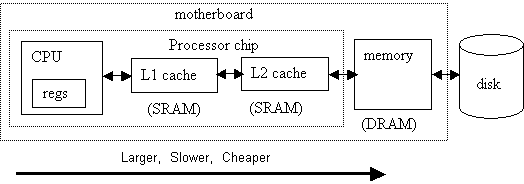
\includegraphics[width=0.8\linewidth]{img/image_2022-11-24-13-17-16.png}
	\caption{Cache and memory hierarchy}
\end{figure}

Caches exploit a common tendency of programs: spatial and temporal \textit{locality}; recently referenced items are likely to be referenced again soon and nearby elements tend to be referenced close together in time.

For example, consider


\begin{listing}[H]
\begin{minted}{c}
for (int i = 0; i < n; i++){
	sum += A[i];
}
\end{minted}
\end{listing}

This snippet displays spatial locality in the data access of the array and temporal locality in that the body of the loop composes a sequence of instructions that will be fetched and executed repeatedly.
By storing a subset of memory into spatially local \textit{blocks}, we can often reduce the amount of disk accesses by having a, well, cached copy available nearby.


Typical processor implementations have separate L1 caches for instructions and data, and a single (larger) L2 cache that is shared between the two.

Some keywords:


\begin{itemize}
	\item cache capacity: the number of bytes the cache can hold
	\item placement: where the cache block should be placed
	\item identification: how to find a block in the cache
	\item cache hit: when the requested block is in the cache
	\item hit rate: total number of hits / total number of accesses
	\item cache miss: when the requested block is not in the cache
	\item miss rate: total number of misses / total number of accesses
	\item replacement: remove block to make room for new block
	\item replacement strategy: how to choose which block to remove
	\item write strategy: how to handle writes to the cache
\end{itemize}


Cache operation usually involves the following steps:

\begin{enumerate}
	\item CPU loads from addr A
	\item If cache hit -> return value at A stored in cache [DONE]
	\item If cache miss -> load block containing A into cache
	\item Place block in cache, replacing another block if necessary
	\item Return value at A stored in cache [DONE]
\end{enumerate}







Since cache is a subset of memory, we need to be able to identify which block of memory we're looking for.
Cache lookups by convention break up the bits of a memory address into the \textit{tag, set index, and offset}. 

\begin{itemize}
	\item \textit{tag} ($ t $) : since multiple locations can map to each cache block, the tag is used to distinguish between them i.e. which memory location currently is cached
	\item \textit{set index} ($ s $): how to locate a block in the cache: index into the array of sets containing blocks in the cache
	\item \textit{offset} $ b $:  which byte within the block we're looking for
\end{itemize}

A \textit{valid bit} is also associated for every block in the cache since a $ 0x0 $ tag is a valid address.



Tag: $ 2^{n_{rows}} \rightsquigarrow \text{tag} = 32-N$.
Note that the number of ways does not have to be a power of 2. We can have a 3-way cache, etc.

\subsubsection{Implementations}


\begin{definition}
	
\textbf{Direct mapped cache}: each memory location maps to a single specific location in the cache.


For a byte-addressable address space of $ 2^n $, then the size of a block is $ B = 2^b $ bytes, the number of sets $ S = 2^S $, and $ S $ is also equal to the total number of cache blocks in the cache; i.e. there is one block per set in cache. Capacity of a direct mapped cache is therefore $ B \cdot  S = 2^{b+s} $ bytes


\begin{example}

	\marginnote{Out of consideration of typing time, the full example will not be typed out and instead I defer the reader to find it \href{https://www.eecg.toronto.edu/~steffan/teaching/permanent/ece243/cache_lecture/}{here}.}


	Consider a 16 bit address space with a direct-mapped cache with $ t = 8, s = 4, b = 4 $.
	The capacity of this cache is $ 2^{s+b} = 256 $ bytes. The number of sets is $ 2^4 = 16 $ and the block size $ b = 2^4 = 16 $.


	\begin{figure}[H]
		\centering
		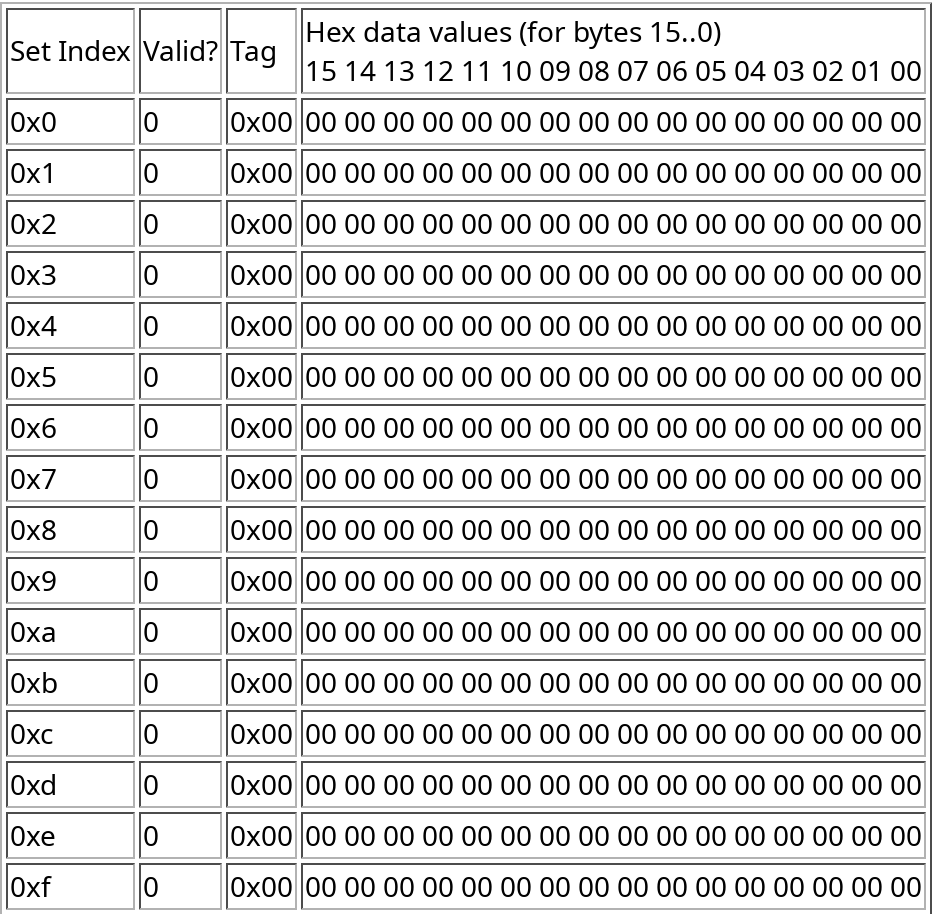
\includegraphics[width=0.8\linewidth]{img/image_2022-11-24-13-50-47.png}
		\caption{Initial cache state}
	\end{figure}


	\texttt{movia r8,0xface; ldb r8,0(r8) }

	\begin{enumerate}
		\item Break address \texttt{0xface} to \texttt{tag = 0xfa}, \texttt{set = 0xc}, \texttt{offset = 0xe}.
		\item The set-index is used to index the cache (\texttt{0xc})
		\item Check the valid bit if the block is valid. Initially this is invalid, so we will have a cache miss.
		\item A request will be made to main memory to load the block containing the address \texttt{0xface}, i.e. the cache block that starts at $ 0xfac0 $ and contains 16 bytes of data between $ 0xfac0 \rightsquigarrow 0xfacf  $
		\item Memory returns the block (after a delay) and the cache set at $ 0xc $ is updated with the new block; the contents are copied over, the valid bit set, and the tag is set equal to $ 0xfa $
		\item Use the offset value $ 0xe $ t index into the cache block and return the requested block
	\end{enumerate}


	A cache hit occurs when the tag matches and the valid bit is set. A more interesting case is a cache miss involving an overwrite.

	Consider 

	






	
\end{example}

\end{definition}






\subsubsection{Handling Writes}

What are ways to handle writes to the cache as to maximize performance i.e. minimize cache misses?


There are two things we can do:
\begin{enumerate}
	\item write something
	\item don't write anything
\end{enumerate}

When do we pick one over the other? Some heuristics include


\begin{enumerate}
	\item  LRU cache: kick the least recently used block out of the cache\mn{Hashmap to doubly linked list, or ring buffer for fixed size}
	\item Random: kick a random block out of the cache
\end{enumerate}










\end{document}

% 352 END

































